\documentclass[11pt,a4paper,oneside]{article}

\usepackage[T1]{fontenc}
\usepackage[utf8]{inputenc}
\IfFileExists{libertinus.sty}{\usepackage{libertinus}}{\usepackage{lmodern}}
\usepackage[final]{microtype}
\usepackage[a4paper,margin=25mm,headheight=15pt]{geometry}
\usepackage{amsmath,amssymb,mathtools,amsthm,mathrsfs,bm}
\usepackage{aliascnt}
\usepackage{booktabs,longtable,tabularx,array,multirow}
\usepackage{graphicx}
\usepackage{caption}
\usepackage{float}
\usepackage{enumitem}
\usepackage{xcolor}
\usepackage{fancyhdr}
\usepackage{listings}
\usepackage{xurl}
\usepackage{hyperref}
\usepackage[nameinlink,capitalise,noabbrev]{cleveref}
\usepackage{bookmark}

\graphicspath{{figures/}}
\allowdisplaybreaks
\setlength{\emergencystretch}{2.5em}
\setcounter{secnumdepth}{3}
\setcounter{tocdepth}{2}
\setlist[itemize]{leftmargin=1.8em,itemsep=0.2em,topsep=0.35em}
\setlist[enumerate]{leftmargin=2.1em,itemsep=0.2em,topsep=0.35em}
\captionsetup{font=small,labelfont=bf}

\definecolor{linkblue}{RGB}{25,75,135}
\definecolor{shadegray}{RGB}{246,247,249}
\definecolor{rulegray}{RGB}{185,191,199}
\hypersetup{
  colorlinks=true,
  linkcolor=linkblue,
  citecolor=linkblue,
  urlcolor=linkblue,
  pdftitle={Interpolation on a Geometric Comb},
  pdfauthor={Research report for Vladimir Reshetnikov's ProveIt project},
  pdfsubject={Lagrange and Newton interpolation, q-analogues, Fabius and Rvachev functions},
  pdfkeywords={geometric interpolation, q-binomial, Jackson derivative, Fabius function, Rvachev up-function, Richardson extrapolation}
}

\pagestyle{fancy}
\fancyhf{}
\fancyhead[L]{\small Interpolation on a geometric comb}
\fancyhead[R]{\small\nouppercase{\leftmark}}
\fancyfoot[C]{\thepage}
\renewcommand{\headrulewidth}{0.4pt}

\newtheorem{theorem}{Theorem}[section]

\newaliascnt{proposition}{theorem}
\newtheorem{proposition}[proposition]{Proposition}
\aliascntresetthe{proposition}
\newaliascnt{lemma}{theorem}
\newtheorem{lemma}[lemma]{Lemma}
\aliascntresetthe{lemma}
\newaliascnt{corollary}{theorem}
\newtheorem{corollary}[corollary]{Corollary}
\aliascntresetthe{corollary}
\newaliascnt{conjecture}{theorem}
\newtheorem{conjecture}[conjecture]{Conjecture}
\aliascntresetthe{conjecture}
\newaliascnt{problem}{theorem}
\newtheorem{problem}[problem]{Problem}
\aliascntresetthe{problem}

\theoremstyle{definition}
\newaliascnt{definition}{theorem}
\newtheorem{definition}[definition]{Definition}
\aliascntresetthe{definition}
\newaliascnt{example}{theorem}
\newtheorem{example}[example]{Example}
\aliascntresetthe{example}
\newaliascnt{algorithm}{theorem}
\newtheorem{algorithm}[algorithm]{Algorithm}
\aliascntresetthe{algorithm}

\theoremstyle{remark}
\newaliascnt{remark}{theorem}
\newtheorem{remark}[remark]{Remark}
\aliascntresetthe{remark}
\newaliascnt{warning}{theorem}
\newtheorem{warning}[warning]{Warning}
\aliascntresetthe{warning}

\crefname{theorem}{Theorem}{Theorems}
\Crefname{theorem}{Theorem}{Theorems}
\crefname{proposition}{Proposition}{Propositions}
\Crefname{proposition}{Proposition}{Propositions}
\crefname{lemma}{Lemma}{Lemmas}
\Crefname{lemma}{Lemma}{Lemmas}
\crefname{corollary}{Corollary}{Corollaries}
\Crefname{corollary}{Corollary}{Corollaries}
\crefname{conjecture}{Conjecture}{Conjectures}
\Crefname{conjecture}{Conjecture}{Conjectures}
\crefname{problem}{Problem}{Problems}
\Crefname{problem}{Problem}{Problems}
\crefname{definition}{Definition}{Definitions}
\Crefname{definition}{Definition}{Definitions}
\crefname{example}{Example}{Examples}
\Crefname{example}{Example}{Examples}
\crefname{algorithm}{Algorithm}{Algorithms}
\Crefname{algorithm}{Algorithm}{Algorithms}
\crefname{remark}{Remark}{Remarks}
\Crefname{remark}{Remark}{Remarks}
\crefname{warning}{Warning}{Warnings}
\Crefname{warning}{Warning}{Warnings}

\newenvironment{statusbox}[1]{%
  \par\smallskip\noindent\begin{center}\begin{minipage}{0.94\textwidth}%
  \hrule\vspace{0.55em}\noindent\textbf{#1}\par\smallskip
}{%
  \vspace{0.55em}\hrule\end{minipage}\end{center}\smallskip
}

\lstdefinestyle{pythonstyle}{
  language=Python,
  basicstyle=\ttfamily\footnotesize,
  backgroundcolor=\color{shadegray},
  frame=single,
  rulecolor=\color{rulegray},
  columns=fullflexible,
  keepspaces=true,
  showstringspaces=false,
  breaklines=true,
  xleftmargin=0.6em,
  xrightmargin=0.6em,
  aboveskip=0.7em,
  belowskip=0.7em
}

\newcommand{\R}{\mathbb R}
\newcommand{\C}{\mathbb C}
\newcommand{\Q}{\mathbb Q}
\newcommand{\Z}{\mathbb Z}
\newcommand{\N}{\mathbb N}
\newcommand{\E}{\mathbb E}
\newcommand{\Prob}{\mathbb P}
\newcommand{\dd}{\,\mathrm d}
\newcommand{\e}{\mathrm e}
\newcommand{\ii}{\mathrm i}
\newcommand{\eps}{\varepsilon}
\newcommand{\bigO}{\mathcal O}
\newcommand{\smallo}{o}
\newcommand{\supp}{\operatorname{supp}}
\newcommand{\Span}{\operatorname{span}}
\newcommand{\diag}{\operatorname{diag}}
\newcommand{\rank}{\operatorname{rank}}
\newcommand{\Up}{\operatorname{up}}
\newcommand{\sincpi}{\operatorname{sinc}_{\pi}}
\newcommand{\Mellin}{\mathcal M}
\newcommand{\Gop}{\mathcal G}
\newcommand{\Iop}{\mathcal I}
\newcommand{\Dq}{D_q}
\newcommand{\Mq}{\mathsf M_q}
\newcommand{\abs}[1]{\left\lvert#1\right\rvert}
\newcommand{\norm}[1]{\left\lVert#1\right\rVert}
\newcommand{\floor}[1]{\left\lfloor#1\right\rfloor}
\newcommand{\ceil}[1]{\left\lceil#1\right\rceil}
\newcommand{\angles}[1]{\left\langle#1\right\rangle}
\newcommand{\qpoch}[3]{\left(#1;#2\right)_{#3}}
\newcommand{\qbinom}[3]{\genfrac{[}{]}{0pt}{}{#1}{#2}_{#3}}
\newcommand{\qint}[2]{\left[#1\right]_{#2}}
\newcommand{\qfac}[2]{\left[#1\right]_{#2}!}
\newcommand{\repo}{\nolinkurl{Analysis/FabiusFunction/docs}}
\DeclareMathOperator{\Res}{Res}
\DeclareMathOperator{\Var}{Var}
\DeclareMathOperator{\ord}{ord}

\title{\bfseries Interpolation on a Geometric Comb\\[0.4em]
\large Lagrange filters, Jackson--Newton series, $q$-analogues,\\
and the Fabius--Rvachev bridge}
\author{Independent research report for Vladimir Reshetnikov's \texttt{ProveIt} project}
\date{30 August 2026}

\begin{document}
\maketitle

\begin{abstract}
Let
\[
  \mathcal C_{a,q}=\{a,aq,aq^2,\ldots\},\qquad a\ne0,\quad 0<q<1,
\]
be a one-sided geometric comb accumulating at the origin.  Polynomial
interpolation on its first $n+1$ teeth is governed exactly by finite
$q$-products.  This report develops that observation into a unified theory.
The geometric Vandermonde matrix factors into a Gaussian Pascal matrix and a
diagonal $q$-factorial matrix; the nodal polynomial is a $q$-Pochhammer
symbol; barycentric weights and arbitrary-target cardinal values have closed
$q$-gamma forms; and the Newton divided differences are precisely normalized
Jackson derivatives,
\[
 f[a,aq,\ldots,aq^k]=\frac{D_q^k f(a)}{[k]_q!}.
\]
The resulting extrapolation operator at the accumulation point is the finite
dilation polynomial
\[
 \mathcal G_{n,q}=\frac1{(q;q)_n}\prod_{j=1}^n(E_q-q^jI),
 \qquad (E_qf)(x)=f(qx).
\]
It is therefore diagonal on Mellin monomials.  For every complex $s$,
\[
 \mathcal G_{n,q}(x^s)\big|_{x=a}
 =a^s q^{ns}\frac{(q^{1-s};q)_n}{(q;q)_n}.
\]
This formula extends the familiar integer moment annihilation to fractional
powers and logarithmic powers and makes the relation with Richardson--Romberg
extrapolation transparent.  The exact variation of the zero-evaluation row is
\[
 \sum_{k=0}^n|\lambda_{n,k}^{(q)}|
 =\frac{(-q;q)_n}{(q;q)_n},
\]
so, for fixed $q<1$, extrapolation to the accumulation point is a regular
summability method even though ordinary interpolation away from the comb can
be violently unstable.

The second half constructs the geometric-uniform family
\[
 X_q=(1-q)\sum_{j\ge0}q^jU_j,
 \qquad U_j\sim\operatorname{Unif}[0,1],
\]
with distribution function $F_q$ and centered density $u_q$.  At $q=1/2$,
$F_q$ is the bounded Fabius function and $u_q$ is Rvachev's up-function.  For
$0<q\le1/2$ we prove the exact comb-moment identity
\[
 F_q(q^n)=\frac{q^{n(n+1)/2}}{(1-q)^n n!}\,\E X_q^n.
\]
At the dyadic point this converts the Fabius interpolation table into an
explicit Gaussian/Mersenne transform of the moment sequence.  If $A_n$ is the
Newton coefficient multiplying $\prod_{r<n}(x-2^{-r})$, then
\[
 A_n=\frac1{(1/2;1/2)_n}
 \sum_{j=0}^n(-1)^j\qbinom nj2\frac{\E X^j}{j!}
 =2^{n(n+1)/2}\sum_{j=0}^n
 \frac{(-1)^j\E X^j}{j!\,\mathfrak M_j\mathfrak M_{n-j}},
\]
where $\mathfrak M_r=\prod_{m=1}^r(2^m-1)$.  The extrapolants at zero converge
superexponentially, with a proved $2^{-n^2/4+O(n)}$ bound.  In sharp contrast,
flatness implies that $\limsup|A_n|^{1/n}=\infty$, and hence the Fabius
Newton interpolants diverge at every nonzero point other than the sampled
powers of $1/2$.  Thus their exact convergence set is the comb together with
its accumulation point.

Finally, the Fourier product
\[
 \widehat u_q(\xi)=\prod_{j\ge0}
 \sincpi\!\left(2(1-q)q^j\xi\right)
\]
is fed back through the same geometric filter.  Away from its zeros this gives
a rapidly convergent reciprocal-product expansion for $1/\widehat u_q$, with
an explicit factorial--Gaussian error bound.  The report also relates the
multiplicative Gaussian filter to dyadic Thue--Morse spline formulas, to exact
finite synthesis by shifted up-functions, and to a collection of concrete
formalization and research problems.  An accompanying Python program verifies
the finite identities exactly, computes Fabius moments through order $80$, and
reproduces all numerical figures.
\end{abstract}

\begin{statusbox}{Provenance and novelty discipline}
The starting monograph already contains the finite geometric Newton formula,
the reversed-Gaussian zero-evaluation row, its natural-number moment law, and
the associated formal power-series filter.  The adjacent repository report on
the Lagrange--Legendre--Rvachev loop treats arbitrary-node Lagrange cardinals
and finite up-atom synthesis.  The present report reorganizes those ingredients
around the geometric comb and adds, with proofs, the Gaussian-Pascal matrix
factorization, arbitrary geometric targets, the exact row-variation formula,
the full complex Mellin symbol, logarithmic-power responses, analytic infinite
Jackson--Newton series, a regular-summability theorem, the superflat
nonconvergence theorem, the geometric-uniform comb-moment formula, the exact
Fabius Gaussian/Mersenne transforms, the quadratic endpoint bound, and the
reciprocal Rvachev product filter.  Claims labeled as conjectures are not used
in any proof.  ``New'' means new relative to the inspected live repository
corpus, not a claim of worldwide priority.
\end{statusbox}

\clearpage
\tableofcontents
\clearpage

\section{Orientation and the four equivalent pictures}
\label{sec:orientation}

\subsection{The geometric comb}

Fix $a\in\C\setminus\{0\}$ and a base $q\in\C$ such that
$q^i\ne q^j$ for the powers under consideration.  The finite geometric comb
of order $n$ is
\[
 \mathcal C_{a,q}^{(n)}=\{x_j=aq^j:0\le j\le n\}.
\]
Most analytic statements below assume $0<q<1$.  Algebraic formulas remain
valid for arbitrary nonzero $q$ until two nodes collide.  An affine comb
$b+aq^j$ is reduced to the present one by the change of variable $x\mapsto
x-b$; keeping $b=0$ exposes the multiplicative structure and the accumulation
point.

Four descriptions of the same interpolation problem will be used repeatedly.

\begin{enumerate}
\item In the original variable $x$, the Newton factors are
      $x-a,x-aq,x-aq^2,\ldots$ and hence are finite $q$-Pochhammer products.
\item In the logarithmic variable $x=a\e^{-t}$ with $q=\e^{-h}$, the nodes are
      the arithmetic grid $t=0,h,2h,\ldots$, while a degree-$n$ polynomial in
      $x$ becomes an exponential polynomial in $t$ spanned by
      $1,\e^{-t},\ldots,\e^{-nt}$.
\item On sequences $f(aq^k)$, interpolation at $x=0$ is a finite polynomial in
      the dilation operator $E_q:f(x)\mapsto f(qx)$.
\item Mellin monomials $x^s$ diagonalize dilations.  The interpolation filter
      consequently has an exact scalar symbol expressed by a $q$-Pochhammer
      quotient.
\end{enumerate}

The first two pictures explain why geometric interpolation was already natural
to Stirling and Schellbach; the third is the language of Richardson and
Romberg extrapolation; the fourth is the most efficient bridge to fractional
powers, endpoint asymptotics, and the Fabius/Rvachev system.  Schoenberg's
historical and numerical account~\cite{Schoenberg1981} explicitly connects
these traditions.

\subsection{Basic notation}

For $n\in\N_0$,
\[
 (z;q)_n=\prod_{r=0}^{n-1}(1-zq^r),
 \qquad
 (z;q)_\infty=\prod_{r=0}^{\infty}(1-zq^r)
\]
when the infinite product converges.  The $q$-integer, $q$-factorial, and
Gaussian coefficient are
\[
 [m]_q=\frac{1-q^m}{1-q},\qquad
 [m]_q!=\prod_{r=1}^m[r]_q=\frac{(q;q)_m}{(1-q)^m},
 \qquad
 \qbinom nkq=\frac{(q;q)_n}{(q;q)_k(q;q)_{n-k}}.
\]
The Gaussian coefficient is set to zero when $k\notin\{0,\ldots,n\}$.  We use
Euler's finite $q$-binomial theorem in the form
\begin{equation}
 (z;q)_n=\sum_{r=0}^n(-1)^rq^{\binom r2}\qbinom nrq z^r.
 \label{eq:finite-qbinomial}
\end{equation}
Standard references for this notation and its analytic continuations are
Gasper--Rahman~\cite{GasperRahman2004}, Kac--Cheung~\cite{KacCheung2002}, and
the DLMF~\cite{DLMF17}.

\subsection{A map of the proved results}

The algebraic core consists of three triangular transforms:
\[
 \text{monomials}
 \longleftrightarrow
 \text{geometric Newton products}
 \longleftrightarrow
 \text{sample values on }\mathcal C_{a,q}^{(n)}.
\]
All three transforms are Gaussian.  The analytic core then separates into two
opposite facts.

\begin{itemize}
\item At the accumulation point, the Lagrange rows have uniformly bounded
      total variation, so they define a regular summability method for every
      continuous germ.
\item Away from the comb, data that are nonzero but flat at the accumulation
      point force superexponential Newton coefficients and divergence.
\end{itemize}

The Fabius function realizes both extremes simultaneously: exact dyadic values
make the Gaussian transforms arithmetic, while endpoint flatness makes the
interpolants converge extraordinarily fast at $0$ and diverge extraordinarily
fast almost everywhere else.

\section{Algebra of the geometric Vandermonde system}
\label{sec:algebra}

\subsection{Nodal polynomial and Vandermonde determinant}

\begin{proposition}[The nodal polynomial is a shifted factorial]
\label{prop:nodal-polynomial}
For the nodes $x_j=aq^j$, $0\le j\le n$, put
\[
 \Omega_{n+1}(x)=\prod_{j=0}^n(x-aq^j).
\]
Then
\begin{align}
 \Omega_{n+1}(x)
 &=x^{n+1}(a/x;q)_{n+1},
 \label{eq:nodal-forward}\\
 &=(-a)^{n+1}q^{\binom{n+1}{2}}(x/a;q^{-1})_{n+1}.
 \label{eq:nodal-reversed}
\end{align}
The geometric Vandermonde determinant is
\begin{equation}
 \prod_{0\le i<j\le n}(aq^j-aq^i)
 =(-1)^{\binom{n+1}{2}}a^{\binom{n+1}{2}}
 q^{\binom{n+1}{3}}
 \prod_{d=1}^n(1-q^d)^{n+1-d}.
 \label{eq:geometric-vandermonde}
\end{equation}
\end{proposition}

\begin{proof}
The first identity is obtained by factoring $x$ from every factor.  For the
second, write
$x-aq^j=-aq^j(1-xq^{-j}/a)$ and multiply the powers of $q$.
For the determinant, each pair contributes
$q^j-q^i=-q^i(1-q^{j-i})$.  There are $n+1-d$ pairs with difference $d$, and
\[
 \sum_{0\le i<j\le n}i
 =\sum_{i=0}^{n-1}i(n-i)=\binom{n+1}{3}.
\]
Multiplication gives \eqref{eq:geometric-vandermonde}.
\end{proof}

\begin{remark}
Formula \eqref{eq:geometric-vandermonde} is already a conditioning warning.
For fixed $n$, it vanishes to order $\binom{n+1}{2}$ as $q\to1$; for fixed
$q<1$, it contains the superexponentially small factor
$q^{\binom{n+1}{3}}$.  These two mechanisms correspond, respectively, to
coalescence of all nodes at $a$ and accumulation of the late nodes at $0$.
\end{remark}

\subsection{The Gaussian Pascal factorization}

Define the geometric Newton products
\begin{equation}
 \Phi_0(x)=1,
 \qquad
 \Phi_k(x)=\prod_{r=0}^{k-1}(x-aq^r)
 =(-a)^kq^{\binom k2}(x/a;q^{-1})_k.
 \label{eq:newton-products}
\end{equation}

\begin{theorem}[Evaluation matrix and Gaussian Pascal matrix]
\label{thm:pascal-factorization}
For $0\le k,j\le n$,
\begin{equation}
 \Phi_k(aq^j)=
 \begin{cases}
 (-a)^kq^{\binom k2}(q;q)_k\qbinom jkq,&j\ge k,\\
 0,&j<k.
 \end{cases}
 \label{eq:newton-evaluation}
\end{equation}
Consequently the lower-triangular evaluation matrix
$V^{\mathrm N}_{j,k}=\Phi_k(aq^j)$ factors as
\begin{equation}
 V^{\mathrm N}=P_qD_{a,q},
 \qquad
 (P_q)_{j,k}=\qbinom jkq,
 \qquad
 (D_{a,q})_{k,k}=(-a)^kq^{\binom k2}(q;q)_k.
 \label{eq:pascal-matrix-factorization}
\end{equation}
The inverse Gaussian Pascal matrix is
\begin{equation}
 (P_q^{-1})_{j,k}
 =(-1)^{j-k}q^{\binom{j-k}{2}}\qbinom jkq
 \qquad (j\ge k).
 \label{eq:q-pascal-inverse}
\end{equation}
\end{theorem}

\begin{proof}
If $j<k$, the product $\Phi_k(aq^j)$ contains its zero factor.  If $j\ge k$,
\begin{align*}
 \Phi_k(aq^j)
 &=\prod_{r=0}^{k-1}\bigl(aq^j-aq^r\bigr)\\
 &=(-a)^kq^{\binom k2}
   \prod_{r=0}^{k-1}(1-q^{j-r})\\
 &=(-a)^kq^{\binom k2}\frac{(q;q)_j}{(q;q)_{j-k}}\\
 &=(-a)^kq^{\binom k2}(q;q)_k\qbinom jkq.
\end{align*}
This proves the factorization.  To verify the inverse, multiply the proposed
matrices.  After the standard Gaussian convolution
\(
 \qbinom jrq\qbinom rkq=\qbinom jkq\qbinom{j-k}{r-k}q
\), the off-diagonal entry is a scalar multiple of
\[
 \sum_{s=0}^{j-k}(-1)^sq^{\binom s2}\qbinom{j-k}{s}q
 =(1;q)_{j-k}=0.
\]
The diagonal entry is $1$.
\end{proof}

\begin{remark}[Why Gaussian coefficients are unavoidable]
The matrix $q^{jm}$ of monomial values on the comb is simultaneously a
Vandermonde matrix and a finite Laplace-transform matrix.  Factoring it through
Newton products produces $P_q$.  Thus Gaussian coefficients do not enter by
analogy or decoration: they are the exact incidence coefficients of the
geometric evaluation map.
\end{remark}

\subsection{Two inverse basis changes}

\begin{theorem}[Monomial--Newton connection coefficients]
\label{thm:basis-change}
For every $k,m\ge0$,
\begin{align}
 \Phi_k(x)
 &=\sum_{j=0}^k(-1)^{k-j}a^{k-j}
 q^{\binom{k-j}{2}}\qbinom kjq x^j,
 \label{eq:newton-to-monomial}\\
 x^m
 &=\sum_{k=0}^m\qbinom mkq a^{m-k}\Phi_k(x).
 \label{eq:monomial-to-newton}
\end{align}
\end{theorem}

\begin{proof}
Expand $x^k(a/x;q)_k$ by \eqref{eq:finite-qbinomial} and put $j=k-r$ to get
\eqref{eq:newton-to-monomial}.  For the inverse, either apply
\eqref{eq:q-pascal-inverse}, or note that the coefficient of $\Phi_k$ in the
Newton interpolant of $x^m$ is its divided difference on
$a,aq,\ldots,aq^k$.  The direct calculation in \Cref{thm:jackson-divided}
below gives $a^{m-k}\qbinom mkq$.
\end{proof}

\begin{corollary}[Newton coefficients of a formal power series]
\label{cor:formal-newton-coefficients}
If $f(x)=\sum_{m\ge0}c_mx^m$ is a formal power series, then its formal
geometric Newton coefficients are
\begin{equation}
 A_k=\sum_{r\ge0}c_{k+r}\qbinom{k+r}{k}q a^r.
 \label{eq:formal-Ak}
\end{equation}
Whenever rearrangement is justified,
$f(x)=\sum_{k\ge0}A_k\Phi_k(x)$.
\end{corollary}

\begin{proof}
Insert \eqref{eq:monomial-to-newton} into each monomial and collect the
coefficient of $\Phi_k$.
\end{proof}

\section{Lagrange cardinal functions on the comb}
\label{sec:lagrange}

\subsection{Barycentric weights}

Let $\ell_{n,j}$ denote the cardinal polynomial satisfying
$\ell_{n,j}(aq^r)=\delta_{jr}$ for $0\le r\le n$.

\begin{theorem}[Closed barycentric weights]
\label{thm:barycentric}
The literal barycentric weights
$\beta_{n,j}=1/\Omega_{n+1}'(aq^j)$ are
\begin{equation}
 \beta_{n,j}
 =\frac{(-1)^jq^{-jn+\binom{j+1}{2}}}
 {a^n(q;q)_j(q;q)_{n-j}}.
 \label{eq:barycentric-weights}
\end{equation}
Their consecutive ratio is
\begin{equation}
 \frac{\beta_{n,j+1}}{\beta_{n,j}}
 =-q^{j+1-n}\frac{1-q^{n-j}}{1-q^{j+1}}.
 \label{eq:barycentric-ratio}
\end{equation}
For $x$ not equal to a node,
\begin{equation}
 (\Iop_nf)(x)=
 \frac{\displaystyle\sum_{j=0}^n
       \frac{\beta_{n,j}f(aq^j)}{x-aq^j}}
      {\displaystyle\sum_{j=0}^n
       \frac{\beta_{n,j}}{x-aq^j}}.
 \label{eq:barycentric-formula}
\end{equation}
\end{theorem}

\begin{proof}
Split the derivative product into indices below and above $j$:
\begin{align*}
 \prod_{\substack{0\le r\le n\\r\ne j}}(aq^j-aq^r)
 &=a^n
 \left[\prod_{r<j}-q^r(1-q^{j-r})\right]
 \left[\prod_{r>j}q^j(1-q^{r-j})\right]\\
 &=a^n(-1)^jq^{jn-\binom{j+1}{2}}
   (q;q)_j(q;q)_{n-j}.
\end{align*}
Taking the reciprocal gives \eqref{eq:barycentric-weights}; division of two
successive terms gives \eqref{eq:barycentric-ratio}.  The barycentric formula
is the usual identity
$\ell_{n,j}(x)=\beta_{n,j}/(x-aq^j)\big/\sum_r\beta_{n,r}/(x-aq^r)$.
\end{proof}

\begin{algorithm}[Stable construction of the weights]
The common scale of barycentric weights cancels in
\eqref{eq:barycentric-formula}.  Set an arbitrary nonzero
$\widetilde\beta_{n,0}$ and generate the rest by
\eqref{eq:barycentric-ratio}, renormalizing the whole row whenever magnitudes
leave a safe floating-point range.  This avoids separately forming
$q^{-jn+\binom{j+1}{2}}$ and the small products $(q;q)_j$.
\end{algorithm}

\subsection{A target on the same multiplicative line}

A target $x=aq^\alpha$, where $\alpha$ need not be integral, preserves all
$q$-structure.

\begin{theorem}[Arbitrary geometric target]
\label{thm:general-target}
Choose a branch of $q^\alpha$.  If $q^\alpha$ is not one of
$1,q,\ldots,q^n$, then
\begin{equation}
 \ell_{n,j}(aq^\alpha)
 =(-1)^{n-j}q^{\binom{n-j+1}{2}}
 \frac{(q^{\alpha-n};q)_{n+1}}
 {(1-q^{\alpha-j})(q;q)_j(q;q)_{n-j}}.
 \label{eq:general-target-cardinal}
\end{equation}
At $\alpha=j$ the singularity is removable and the value is $1$; at every
other integral node it is $0$.  For $0<q<1$ and
$\Re\alpha\to+\infty$, the weights tend to the zero-target row
\begin{equation}
 \lambda_{n,j}^{(q)}
 =\ell_{n,j}(0)
 =\frac{(-1)^{n-j}q^{\binom{n-j+1}{2}}}
 {(q;q)_j(q;q)_{n-j}}.
 \label{eq:zero-target-row}
\end{equation}
\end{theorem}

\begin{proof}
Use
$\ell_{n,j}(x)=\Omega_{n+1}(x)/((x-aq^j)\Omega'_{n+1}(aq^j))$,
\Cref{prop:nodal-polynomial}, and \eqref{eq:barycentric-weights}.  The product
at the target is
\[
 \prod_{r=0}^n(q^\alpha-q^r)
 =(-1)^{n+1}q^{\binom{n+1}{2}}(q^{\alpha-n};q)_{n+1}.
\]
Extracting $-q^j$ from $q^\alpha-q^j$ leaves exactly
\eqref{eq:general-target-cardinal}.  The limiting assertions follow directly
from the product.
\end{proof}

\begin{remark}[$q$-gamma form]
Since
\[
 (q^{\alpha-n};q)_{n+1}
 =(1-q)^{n+1}\frac{\Gamma_q(\alpha+1)}{\Gamma_q(\alpha-n)},
\]
formula \eqref{eq:general-target-cardinal} is meromorphic in $\alpha$ and can
be rewritten entirely with $q$-gamma functions and the $q$-number
$[\alpha-j]_q$.  This is the natural analytic continuation of the cardinal
row, not merely a formal replacement of factorials by $q$-factorials.
\end{remark}

\subsection{The zero row as a dilation polynomial}

\begin{theorem}[Reversed Gaussian characteristic identity]
\label{thm:filter-characteristic}
For every indeterminate $z$,
\begin{equation}
 \sum_{k=0}^n\lambda_{n,k}^{(q)}z^k
 =\frac1{(q;q)_n}\prod_{j=1}^n(z-q^j).
 \label{eq:lambda-characteristic}
\end{equation}
Consequently, with $(E_qf)(x)=f(qx)$,
\begin{equation}
 (\Gop_{n,q}f)(x)
 :=\sum_{k=0}^n\lambda_{n,k}^{(q)}f(q^kx)
 =\frac1{(q;q)_n}\prod_{j=1}^n(E_q-q^jI)f(x).
 \label{eq:dilation-filter}
\end{equation}
The operator reproduces constants and annihilates $x,x^2,\ldots,x^n$.
\end{theorem}

\begin{proof}
Expand the product after reversing the finite $q$-binomial theorem.  More
explicitly, the coefficient of $z^k$ in
$\prod_{j=1}^n(z-q^j)$ is
\[
 (-1)^{n-k}q^{\binom{n-k+1}{2}}\qbinom nkq,
\]
and division by $(q;q)_n$ gives \eqref{eq:zero-target-row}.  Substitution of
$E_q$ for $z$ proves \eqref{eq:dilation-filter}.  On $x^d$, $E_q$ has
eigenvalue $q^d$, so one factor vanishes when $1\le d\le n$; the value on a
constant is $1$.
\end{proof}

\begin{remark}[Denominator-free form]
Multiplying \eqref{eq:lambda-characteristic} by $(q;q)_n$ produces an identity
in $\Z[q,z]$.  It remains meaningful at roots of unity even when the normalized
Lagrange row is undefined because nodes collide.  This denominator-free
residual is the right starting point for confluent and cyclotomic versions of
the theory.
\end{remark}

\subsection{Exact total variation and conditioning at the accumulation point}

\begin{theorem}[Exact row norm]
\label{thm:row-norm}
For $0<q<1$,
\begin{equation}
 \sum_{k=0}^n\abs{\lambda_{n,k}^{(q)}}
 =\frac{(-q;q)_n}{(q;q)_n}
 =\prod_{j=1}^n\frac{1+q^j}{1-q^j}.
 \label{eq:row-norm}
\end{equation}
In particular the row norms increase to the finite limit
\begin{equation}
 K(q)=\frac{(-q;q)_\infty}{(q;q)_\infty}.
 \label{eq:row-norm-limit}
\end{equation}
For fixed $n$ and $q\to1^-$,
\begin{equation}
 \sum_{k=0}^n\abs{\lambda_{n,k}^{(q)}}
 \sim\frac{2^n}{n!(1-q)^n}.
 \label{eq:finite-row-q1}
\end{equation}
If $q=\e^{-h}$ and $h\to0^+$, then
\begin{equation}
 K(\e^{-h})
 \sim\frac{\sqrt h}{2\sqrt\pi}
 \exp\!\left(\frac{\pi^2}{4h}\right).
 \label{eq:infinite-row-q1}
\end{equation}
\end{theorem}

\begin{proof}
Because the signs alternate,
\begin{align*}
 \sum_{k=0}^n|\lambda_{n,k}^{(q)}|
 &=\frac1{(q;q)_n}\sum_{r=0}^n
 q^{\binom{r+1}{2}}\qbinom nrq\\
 &=\frac{(-q;q)_n}{(q;q)_n},
\end{align*}
where $r=n-k$ and the last step is the finite $q$-binomial theorem applied to
$\prod_{j=1}^n(1+q^j)$.  The infinite product converges for $q<1$.
For fixed $n$, use $1-q^j\sim j(1-q)$ and $1+q^j\sim2$.
Finally,
\[
 \frac{(-q;q)_\infty}{(q;q)_\infty}
 =\frac{(q^2;q^2)_\infty}{(q;q)_\infty^2}.
\]
The standard Dedekind--eta asymptotic
$(\e^{-h};\e^{-h})_\infty\sim
\sqrt{2\pi/h}\exp(-\pi^2/(6h)+h/24)$ gives
\eqref{eq:infinite-row-q1} after substitution at $h$ and $2h$.
\end{proof}

\begin{remark}
The finite condition number blows up when $q$ approaches $1$, but for every
fixed $q<1$ the entire sequence of extrapolation rows has bounded variation.
This distinction is essential.  The accumulation point is stable as a
summability target at fixed ratio, even though coalescing ratios are extremely
ill-conditioned.
\end{remark}

\section{Mellin symbols and exact residuals}
\label{sec:mellin}

\subsection{Complex powers}

The integer moment law in the source monograph is one specialization of a
stronger identity.  Since dilations act diagonally on every chosen branch of
$x^s$, the full spectral response is available at once.

\begin{theorem}[Exact Mellin symbol]
\label{thm:mellin-symbol}
Let $s\in\C$, choose a branch of $a^s$ and $q^s$, and set
\begin{equation}
 M_{n,q}(s)=\sum_{k=0}^n\lambda_{n,k}^{(q)}q^{ks}.
 \label{eq:mellin-symbol-definition}
\end{equation}
Then
\begin{align}
 M_{n,q}(s)
 &=\frac{\prod_{j=1}^n(q^s-q^j)}{(q;q)_n}
 \label{eq:mellin-product}\\
 &=q^{ns}\frac{(q^{1-s};q)_n}{(q;q)_n}
 \label{eq:mellin-forward}\\
 &=(-1)^nq^{\binom{n+1}{2}}
   \frac{(q^{s-n};q)_n}{(q;q)_n}.
 \label{eq:mellin-reversed}
\end{align}
Equivalently,
\begin{equation}
 (\Gop_{n,q}x^s)(a)=a^sM_{n,q}(s).
 \label{eq:mellin-eigenvalue}
\end{equation}
The zeros at $s=1,\ldots,n$ are simple modulo the imaginary period
$2\pi\ii/\log q$.
\end{theorem}

\begin{proof}
Evaluate \eqref{eq:lambda-characteristic} at $z=q^s$.  Factoring $q^s$ from
each factor gives \eqref{eq:mellin-forward}; factoring $-q^j$ gives
\eqref{eq:mellin-reversed}.
\end{proof}

\begin{corollary}[Natural moments and the first residual]
\label{cor:integer-moments}
For $d\in\N_0$,
\begin{equation}
 \sum_{k=0}^n\lambda_{n,k}^{(q)}q^{kd}
 =\begin{cases}
 1,&d=0,\\
 0,&1\le d\le n,\\
 (-1)^nq^{\binom{n+1}{2}}\qbinom{d-1}{n}q,&d\ge n+1.
 \end{cases}
 \label{eq:integer-moment-law}
\end{equation}
\end{corollary}

\begin{proof}
The first two cases follow from the zeros in
\eqref{eq:mellin-product}.  For $d\ge n+1$,
\[
 (q^{d-n};q)_n=\frac{(q;q)_{d-1}}{(q;q)_{d-n-1}},
\]
and substitution into \eqref{eq:mellin-reversed} gives the Gaussian
coefficient.
\end{proof}

\begin{remark}[Fractional endpoint laws]
For fixed $s$ with $\Re s>0$ and $s\notin\N$,
\begin{equation}
 M_{n,q}(s)
 \sim q^{ns}\frac{(q^{1-s};q)_\infty}{(q;q)_\infty}
 \qquad(n\to\infty).
 \label{eq:fractional-asymptotic}
\end{equation}
Thus a fractional power $x^s$ is not annihilated, but its extrapolation error
has a completely explicit geometric rate.  Integer powers are exceptional
because the finite product terminates at an exact zero.
\end{remark}

\subsection{Logarithmic powers by spectral differentiation}

Differentiate \eqref{eq:mellin-eigenvalue} with respect to $s$.  This gives
closed responses for singular terms common in endpoint asymptotics.

\begin{proposition}[Powers times logarithms]
\label{prop:log-powers}
For every integer $r\ge0$,
\begin{equation}
 \sum_{k=0}^n\lambda_{n,k}^{(q)}(aq^k)^s
 \bigl(\log a+k\log q\bigr)^r
 =\frac{\partial^r}{\partial s^r}\bigl(a^sM_{n,q}(s)\bigr).
 \label{eq:log-power-response}
\end{equation}
In particular, if $1\le d\le n$, then
\begin{equation}
 \sum_{k=0}^n\lambda_{n,k}^{(q)}(aq^k)^d\log(aq^k)
 =a^dM_{n,q}'(d),
 \label{eq:first-log-response}
\end{equation}
where
\begin{equation}
 M_{n,q}'(d)
 =(-1)^{d-1}(\log q)
 q^{d(2n-d+1)/2}
 \frac{(q;q)_{d-1}(q;q)_{n-d}}{(q;q)_n}.
 \label{eq:mellin-derivative-integer}
\end{equation}
\end{proposition}

\begin{proof}
Termwise differentiation is legitimate because the sum is finite.  At
$s=d$, the factor $q^s-q^d$ is the unique vanishing factor in
\eqref{eq:mellin-product}.  Differentiating that factor and splitting the
remaining product below and above $d$ gives
\begin{align*}
 q^d\log q\prod_{\substack{1\le j\le n\\j\ne d}}(q^d-q^j)
 &=(-1)^{d-1}(\log q)
 q^{d(2n-d+1)/2}(q;q)_{d-1}(q;q)_{n-d}.
\end{align*}
Division by $(q;q)_n$ proves \eqref{eq:mellin-derivative-integer}.
\end{proof}

\begin{remark}
A filter that is exact on polynomials need not suppress logarithmic
corrections attached to those powers.  Formula
\eqref{eq:mellin-derivative-integer} quantifies the leakage exactly.  Higher
$s$-derivatives introduce finite sums of $q$-harmonic terms
$(1-q^j)^{-r}$ and can be organized with complete Bell polynomials.
\end{remark}

\subsection{Mellin-transform interpretation}

For a function on $(0,\infty)$ with Mellin transform
\[
 (\Mellin f)(z)=\int_0^\infty f(x)x^{z-1}\dd x,
\]
one has
\[
 \Mellin[f(q^kx)](z)=q^{-kz}(\Mellin f)(z).
\]
Hence, on a common strip of convergence,
\begin{equation}
 \Mellin[\Gop_{n,q}f](z)=M_{n,q}(-z)(\Mellin f)(z).
 \label{eq:mellin-transform-multiplier}
\end{equation}
The geometric Lagrange filter is therefore a finite Mellin multiplier.  Its
spectral zeros are the same integer moments that the interpolation formula
annihilates in physical space.  This is the multiplicative analogue of an
ordinary finite-difference stencil whose Fourier symbol has a prescribed zero
at the origin.

\subsection{The universal complete-symmetric residual}

Let $v_0,\ldots,v_n$ be arbitrary distinct nodes and let
$h_r(z_0,\ldots,z_m)$ denote the complete homogeneous symmetric polynomial of
degree $r$.  The following identity specializes particularly cleanly on a
geometric comb.

\begin{theorem}[Exact monomial residual]
\label{thm:universal-residual}
Let $\ell_j$ be the Lagrange cardinal functions for
$v_0,\ldots,v_n$, and put $\Omega(x)=\prod_{j=0}^n(x-v_j)$.  For every
$r\ge0$,
\begin{equation}
 x^{n+1+r}-\sum_{j=0}^n\ell_j(x)v_j^{n+1+r}
 =\Omega(x)h_r(x,v_0,\ldots,v_n).
 \label{eq:universal-residual}
\end{equation}
On $v_j=aq^j$,
\begin{equation}
 h_r(x,a,aq,\ldots,aq^n)
 =\sum_{s=0}^r x^s a^{r-s}\qbinom{n+r-s}{n}q.
 \label{eq:geometric-complete-h}
\end{equation}
\end{theorem}

\begin{proof}
The left side of \eqref{eq:universal-residual} vanishes at every node, hence is
divisible by $\Omega$.  Both sides are homogeneous of total degree $n+1+r$
in $x,v_0,\ldots,v_n$.  The quotient is identified from the generating
function
\[
 \sum_{r\ge0}h_r(x,v_0,\ldots,v_n)t^r
 =\frac1{(1-xt)\prod_{j=0}^n(1-v_jt)}.
\]
Equivalently, polynomial division of $x^{n+1+r}$ by $\Omega$ gives the same
recurrence.  At geometric nodes,
\[
 \prod_{j=0}^n\frac1{1-aq^jt}
 =\sum_{m\ge0}\qbinom{n+m}{n}q a^mt^m
\]
by the reciprocal finite $q$-binomial theorem.  Multiplication by
$(1-xt)^{-1}$ and extraction of $t^r$ proves
\eqref{eq:geometric-complete-h}.
\end{proof}

\begin{corollary}[Exact analytic interpolation tail]
\label{cor:analytic-residual}
Let $f(x)=\sum_{m\ge0}c_mx^m$ converge absolutely in a disk containing the
nodes and the target.  Then
\begin{equation}
 f(x)-(\Iop_nf)(x)
 =\Omega_{n+1}(x)
 \sum_{r\ge0}c_{n+1+r}
 \sum_{s=0}^r x^sa^{r-s}\qbinom{n+r-s}{n}q.
 \label{eq:analytic-residual}
\end{equation}
At $x=0$ this becomes
\begin{equation}
 (\Gop_{n,q}f)(a)-f(0)
 =(-1)^n a^{n+1}q^{\binom{n+1}{2}}
 \sum_{r\ge0}c_{n+1+r}a^r\qbinom{n+r}{n}q.
 \label{eq:zero-analytic-tail}
\end{equation}
\end{corollary}

\begin{proof}
Sum \eqref{eq:universal-residual} over the monomial coefficients.  Absolute
convergence justifies rearrangement.  Since
$\Omega_{n+1}(0)=(-a)^{n+1}q^{\binom{n+1}{2}}$, moving the residual to the
other side gives \eqref{eq:zero-analytic-tail}.
\end{proof}

\begin{corollary}[A disk bound]
\label{cor:disk-bound}
Suppose $f$ is analytic on $|z|<R$ and $|f(z)|\le B$ on $|z|=R$.  If
$|a|<R$, then
\begin{equation}
 \abs{(\Gop_{n,q}f)(a)-f(0)}
 \le
 \frac{Bq^{\binom{n+1}{2}}}{(q;q)_n}
 \frac{(|a|/R)^{n+1}}{1-|a|/R}.
 \label{eq:disk-filter-bound}
\end{equation}
\end{corollary}

\begin{proof}
Cauchy's estimate gives $|c_m|\le BR^{-m}$, and
$\qbinom{n+r}{n}q\le1/(q;q)_n$ for $0<q<1$.  Apply these estimates to
\eqref{eq:zero-analytic-tail} and sum the geometric series.
\end{proof}

\section{Newton interpolation is Jackson calculus}
\label{sec:jackson}

\subsection{Divided differences and iterated \texorpdfstring{$q$}{q}-derivatives}

Use the Jackson derivative convention
\begin{equation}
 (D_qf)(x)=\frac{f(x)-f(qx)}{(1-q)x}.
 \label{eq:jackson-definition}
\end{equation}
It satisfies $D_qx^m=[m]_qx^{m-1}$.

\begin{theorem}[Geometric divided differences are Jackson derivatives]
\label{thm:jackson-divided}
For every polynomial $f$, and more generally whenever all quantities are
defined,
\begin{equation}
 f[a,aq,\ldots,aq^k]
 =\frac{D_q^kf(a)}{[k]_q!}.
 \label{eq:jackson-divided}
\end{equation}
Equivalently,
\begin{align}
 \frac{D_q^kf(a)}{[k]_q!}
 &=\frac1{a^k}
 \sum_{j=0}^k
 \frac{(-1)^jq^{-jk+\binom{j+1}{2}}}
 {(q;q)_j(q;q)_{k-j}}f(aq^j)
 \label{eq:jackson-explicit}\\
 &=\frac1{a^k(q;q)_k}
 \sum_{j=0}^k(-1)^jq^{-jk+\binom{j+1}{2}}
 \qbinom kjq f(aq^j).
 \label{eq:jackson-explicit-qbinom}
\end{align}
\end{theorem}

\begin{proof}
Let $E_qf(x)=f(qx)$.  Because $E_qx^{-1}=q^{-1}x^{-1}E_q$,
iteration of \eqref{eq:jackson-definition} gives the operator identity
\begin{equation}
 D_q^k
 =\frac{x^{-k}}{(1-q)^k}
 \prod_{r=0}^{k-1}(1-q^{-r}E_q).
 \label{eq:jackson-operator-product}
\end{equation}
Expand the product with the finite $q^{-1}$-binomial theorem and use
\(
 \qbinom kj{q^{-1}}=q^{-j(k-j)}\qbinom kjq
\).  Division by
$[k]_q!=(q;q)_k/(1-q)^k$ yields
\eqref{eq:jackson-explicit-qbinom}.  On the other hand, the explicit formula
for a divided difference is
\[
 f[a,aq,\ldots,aq^k]
 =\sum_{j=0}^k
 \frac{f(aq^j)}{\prod_{r\ne j}(aq^j-aq^r)}.
\]
The denominator calculation from \Cref{thm:barycentric}, with $n=k$, is
exactly \eqref{eq:jackson-explicit}.
\end{proof}

\begin{corollary}[Finite Jackson--Newton formula]
\label{cor:finite-jackson-newton}
The degree-$n$ interpolant is
\begin{equation}
 (\Iop_nf)(x)
 =\sum_{k=0}^n\frac{D_q^kf(a)}{[k]_q!}
   \prod_{r=0}^{k-1}(x-aq^r).
 \label{eq:finite-jackson-newton}
\end{equation}
For $f(x)=x^m$, the coefficient is
\begin{equation}
 \frac{D_q^kx^m|_{x=a}}{[k]_q!}
 =\qbinom mkq a^{m-k},
 \label{eq:monomial-jackson}
\end{equation}
which recovers \eqref{eq:monomial-to-newton}.
\end{corollary}

\begin{remark}
The phrase ``$q$-Taylor formula'' can obscure the geometry.  Formula
\eqref{eq:finite-jackson-newton} is literally the ordinary Newton formula on
the nodes $a,aq,\ldots$; Jackson calculus appears because those divided
differences happen to close under dilation.  This also fixes normalization
ambiguities between the several $q$-derivative conventions in the literature.
\end{remark}

\subsection{Infinite Jackson--Newton series for analytic functions}

\begin{theorem}[Local analytic convergence]
\label{thm:infinite-jackson-newton}
Let $0<q<1$, and let $f(z)=\sum_{m\ge0}c_mz^m$ be analytic in $|z|<R$.
If $|a|<R$, define
\begin{equation}
 A_k=\frac{D_q^kf(a)}{[k]_q!}
 =\sum_{r\ge0}c_{k+r}\qbinom{k+r}{k}q a^r.
 \label{eq:analytic-Ak}
\end{equation}
Then
\begin{equation}
 f(x)=\sum_{k=0}^\infty A_k\Phi_k(x)
 \label{eq:infinite-jackson-newton}
\end{equation}
locally uniformly for $|x|<R$.  At the accumulation point,
\begin{equation}
 f(0)=\sum_{k=0}^\infty
 (-a)^kq^{\binom k2}\frac{D_q^kf(a)}{[k]_q!}.
 \label{eq:q-extrapolation-series}
\end{equation}
\end{theorem}

\begin{proof}
Fix $s<R$ and choose $\rho$ with
$\max(s,|a|)<\rho<R$.  Cauchy's estimate gives
$|c_m|\le C\rho^{-m}$.  Since
$\qbinom{k+r}{k}q\le1/(q;q)_\infty$,
\[
 |A_k|\le C_1\rho^{-k}.
\]
For $0<s<R$ and $|x|\le s$,
\[
 |\Phi_k(x)|
 \le\prod_{r=0}^{k-1}(s+|a|q^r)
 \le s^k\prod_{r=0}^\infty(1+|a|q^r/s)=C_2(s)s^k.
\]
Thus the series converges uniformly on $|x|\le s$.  The formal basis identity
in \Cref{cor:formal-newton-coefficients} then identifies its sum with $f$.
At $x=0$, $\Phi_k(0)=(-a)^kq^{\binom k2}$, which proves
\eqref{eq:q-extrapolation-series}.
\end{proof}

\begin{remark}[No analyticity hypothesis can be silently dropped]
The infinite series in \eqref{eq:infinite-jackson-newton} is much more rigid
than the finite interpolation formula.  The Fabius function is $C^\infty$ but
flat at the origin and nowhere analytic; in \Cref{sec:superflat} we prove that
its corresponding infinite Newton series diverges at every off-comb nonzero
point.
\end{remark}

\subsection{The limits \texorpdfstring{$q\to1$}{q to 1} and \texorpdfstring{$q\to0$}{q to 0}}

\begin{proposition}[Taylor limit]
\label{prop:taylor-limit}
For fixed $k$, as $q\to1$,
\[
 D_q^kf(a)\longrightarrow f^{(k)}(a),
 \qquad [k]_q!\longrightarrow k!,
 \qquad \Phi_k(x)\longrightarrow(x-a)^k.
\]
Thus \eqref{eq:finite-jackson-newton} tends termwise to the ordinary Taylor
polynomial about $a$.
\end{proposition}

\begin{proof}
The first statement follows by repeated use of the standard Jackson derivative
limit on a sufficiently differentiable function; the other two are immediate
from their finite products.
\end{proof}

At the opposite endpoint, $D_0f(x)=(f(x)-f(0))/x$ is a tail-quotient operator.
For $f(x)=\sum c_mx^m$,
\[
 \lim_{q\to0}\frac{D_q^kf(a)}{[k]_q!}
 =\sum_{r\ge0}c_{k+r}a^r,
 \qquad
 \lim_{q\to0}\Phi_k(x)=
 \begin{cases}
 1,&k=0,\\
 (x-a)x^{k-1},&k\ge1.
 \end{cases}
\]
The limiting expansion telescopes.  It is not Hermite interpolation at a
multiple node: the geometric rates retain ordered information about how the
nodes approach zero.  A genuine confluent theory requires a further
renormalization and is listed as \Cref{prob:q0-confluent}.

\subsection{Neville, Richardson, and Romberg recurrences}

\begin{theorem}[Geometric Neville recurrence]
\label{thm:neville}
For $i,m\ge0$, let $P_{i,m}$ be the interpolant characterized by
\[
 P_{i,m}(aq^{i+r})=f(aq^{i+r})\qquad(0\le r\le m).
\]
Then
\begin{equation}
 P_{i,m}(x)=
 \frac{(x-aq^{i+m})P_{i,m-1}(x)
      -(x-aq^i)P_{i+1,m-1}(x)}
      {aq^i-aq^{i+m}}.
 \label{eq:geometric-neville}
\end{equation}
At $x=0$, with $R_i^{(0)}=f(aq^i)$,
\begin{equation}
 R_i^{(m)}
 =\frac{R_{i+1}^{(m-1)}-q^mR_i^{(m-1)}}{1-q^m},
 \qquad
 R_0^{(n)}=(\Gop_{n,q}f)(a).
 \label{eq:richardson-recurrence}
\end{equation}
\end{theorem}

\begin{proof}
The numerator in \eqref{eq:geometric-neville} has degree at most $m$ and takes
the required values at both endpoint nodes and all shared interior nodes;
uniqueness proves the formula.  Substitute $x=0$ and cancel $aq^i$.
\end{proof}

\begin{corollary}[Generalized Richardson cancellation]
\label{cor:richardson}
Suppose approximations at scales $h_i=h_0r^i$ have an expansion
\[
 T(h)=L+c_1h^\rho+c_2h^{2\rho}+\cdots.
\]
Apply \eqref{eq:richardson-recurrence} with $q=r^\rho$ to the data $T(h_i)$.
After $n$ levels, the first $n$ error powers are annihilated exactly.  Romberg
quadrature is the special case in which the trapezoidal error uses even powers
and hence $q=r^2$.
\end{corollary}

\begin{remark}
This recurrence is often numerically preferable to forming the closed weights.
It also explains the historical term ``deferred approach to the limit'': each
new level eliminates one Mellin eigenmode of the asymptotic error.
\end{remark}

\section{Convergence at an accumulation point and divergence away from it}
\label{sec:superflat}

\subsection{The zero row is a regular summability method}

\begin{theorem}[Regularity at the accumulation point]
\label{thm:regular-summability}
Let $0<q<1$ and let $y_k\to L$.  Then
\begin{equation}
 \sum_{k=0}^n\lambda_{n,k}^{(q)}y_k\longrightarrow L.
 \label{eq:regular-summability}
\end{equation}
Equivalently, if $f$ is continuous at $0$, the interpolating polynomial through
$(aq^k,f(aq^k))$, $0\le k\le n$, satisfies
\begin{equation}
 (\Iop_nf)(0)\longrightarrow f(0).
 \label{eq:continuous-zero-convergence}
\end{equation}
\end{theorem}

\begin{proof}
The rows reproduce constants by \eqref{eq:integer-moment-law}; their
$\ell^1$ norms are bounded by $K(q)$ by \Cref{thm:row-norm}; and for each fixed
$k$,
\[
 |\lambda_{n,k}^{(q)}|
 =\frac{q^{\binom{n-k+1}{2}}}
 {(q;q)_k(q;q)_{n-k}}\longrightarrow0.
\]
These are precisely the Toeplitz regularity conditions.  For completeness,
subtract $L$, split the sum at a fixed $K$, make the tail small using the
bounded row norm, and then let $n\to\infty$ in the finite head.
\end{proof}

\subsection{The limiting profile viewed from the finest tooth}

Reindex the row by $r=n-k$.  For each fixed $r$,
\begin{equation}
 \lambda_{n,n-r}^{(q)}
 \longrightarrow
 \mu_r^{(q)}
 :=\frac{(-1)^rq^{\binom{r+1}{2}}}
 {(q;q)_\infty(q;q)_r}.
 \label{eq:limiting-row-profile}
\end{equation}
Euler's infinite theorem gives the generating function
\begin{equation}
 \sum_{r=0}^\infty\mu_r^{(q)}z^r
 =\frac{(qz;q)_\infty}{(q;q)_\infty},
 \qquad
 \sum_{r=0}^\infty\mu_r^{(q)}=1.
 \label{eq:limiting-profile-generating}
\end{equation}
Thus the mass does not remain attached to any fixed physical node; it travels
with the finest scale $aq^n$ and approaches a signed, absolutely summable
profile in the reversed index.  This is the mechanism behind
\Cref{thm:regular-summability}.

\subsection{Power, Puiseux, and logarithmic endpoint expansions}

Suppose a germ has a convergent or asymptotic expansion
\[
 f(x)=L+\sum_{r}c_rx^{\alpha_r}(\log x)^{m_r},
 \qquad \Re\alpha_r>0.
\]
Theorems \ref{thm:mellin-symbol} and \ref{prop:log-powers} give the filter of
each term exactly.  In particular, a nonintegral leading exponent $\alpha$
produces the rate $q^{n\alpha}$ times an explicit $q$-product, while an
integral polynomial jet is deleted once $n$ reaches its degree.  The filter is
therefore an endpoint asymptotic microscope: its decay rate distinguishes
fractional regularity from an analytic integer jet.

\begin{proposition}[A simple Hölder estimate]
\label{prop:holder-filter}
If $|f(x)-f(0)|\le C|x|^\alpha$ on the comb, with $\alpha>0$, then
\begin{equation}
 |(\Gop_{n,q}f)(a)-f(0)|
 \le C|a|^\alpha
 \sum_{k=0}^n|\lambda_{n,k}^{(q)}|q^{k\alpha}.
 \label{eq:holder-bound}
\end{equation}
For fixed $q$ and $\alpha$, the right side is $O(q^{n\alpha})$.
\end{proposition}

\begin{proof}
The first statement is the triangle inequality.  Reindex $r=n-k$.  Since
$(q;q)_m\ge(q;q)_\infty$ for every $m$, one has
\begin{align*}
 q^{-n\alpha}
 \sum_{k=0}^n|\lambda_{n,k}^{(q)}|q^{k\alpha}
 &=\sum_{r=0}^n
 \frac{q^{\binom{r+1}{2}-r\alpha}}
 {(q;q)_{n-r}(q;q)_r}\\
 &\le \frac1{(q;q)_\infty^2}
 \sum_{r=0}^\infty q^{\binom{r+1}{2}-r\alpha}<\infty.
\end{align*}
The last series converges for every fixed $\alpha$ because its exponent is
quadratic in $r$.  This uniform bound proves the stated $O(q^{n\alpha})$
estimate.  Dominated convergence also gives the sharper limit
\[
 q^{-n\alpha}
 \sum_{k=0}^n|\lambda_{n,k}^{(q)}|q^{k\alpha}
 \longrightarrow
 \sum_{r=0}^\infty|\mu_r^{(q)}|q^{-r\alpha}.
\]
\end{proof}

\subsection{Superflat data force divergence off the comb}

The favorable result at $0$ has a nearly opposite counterpart everywhere
else.  It is useful to formulate it directly for data, without assuming that
they initially came from a function.

\begin{definition}
A sequence $y_j\to L$ is \emph{$q$-superflat at its limit} if
\begin{equation}
 y_j-L=o(q^{mj})\qquad(j\to\infty)
 \label{eq:q-superflat}
\end{equation}
for every $m\in\N$.
\end{definition}

\begin{theorem}[Exact convergence set for nontrivial superflat data]
\label{thm:superflat-divergence}
Let $0<q<1$, $a\ne0$, and let $y_j\to L$ be $q$-superflat.  Assume
$y_j\ne L$ for infinitely many $j$.  Let
\begin{equation}
 P_n(x)=\sum_{k=0}^n A_k\Phi_k(x)
 \label{eq:superflat-newton}
\end{equation}
be the polynomial interpolating $P_n(aq^j)=y_j$ for $0\le j\le n$.  Then
\begin{equation}
 \limsup_{k\to\infty}|A_k|^{1/k}=\infty.
 \label{eq:superexponential-A}
\end{equation}
Moreover:
\begin{enumerate}
\item $P_n(0)\to L$;
\item for each $m\ge0$, $P_n(aq^m)=y_m$ once $n\ge m$;
\item for every $x\in\C\setminus(\{0\}\cup\{aq^m:m\ge0\})$, the increments
      $A_n\Phi_n(x)$ fail to tend to zero, and the sequence $P_n(x)$ diverges;
      indeed it is unbounded along a subsequence.
\end{enumerate}
Thus the convergence set is exactly the geometric comb together with its
accumulation point.
\end{theorem}

\begin{proof}
Subtract $L$; this changes only $A_0$ and reduces to $L=0$.  Suppose, contrary
to \eqref{eq:superexponential-A}, that $|A_k|\le CR^{-k}$ for some $R>0$.
For every $0<r<R$, the estimate
\[
 \sup_{|z|\le r}|\Phi_k(z)|
 \le r^k\prod_{j=0}^\infty(1+|a|q^j/r)
\]
shows that $g(z)=\sum_{k\ge0}A_k\Phi_k(z)$ is analytic on $|z|<R$.
For every sufficiently large $j$, $|aq^j|<R$, and all terms with $k>j$
vanish at $aq^j$.  Hence
\[
 g(aq^j)=P_j(aq^j)=y_j.
\]
If the first nonzero Taylor coefficient of $g$ at $0$ had order $m$, then
$g(aq^j)/(aq^j)^m$ would tend to a nonzero constant.  This contradicts
$q$-superflatness.  Therefore every Taylor coefficient vanishes, so $g$ is
identically zero near $0$, contradicting the assumption that infinitely many
$y_j$ are nonzero.  This proves \eqref{eq:superexponential-A}.

Assertion 1 is \Cref{thm:regular-summability}, and assertion 2 is interpolation.
For a point $x$ in assertion 3,
\begin{equation}
 \Phi_n(x)=x^n\prod_{r=0}^{n-1}\left(1-\frac{aq^r}{x}\right).
 \label{eq:basis-fixed-x}
\end{equation}
The infinite product tends to $(a/x;q)_\infty\ne0$, because $x$ is not a
node.  Hence $|\Phi_n(x)|^{1/n}\to|x|>0$.  Together with
\eqref{eq:superexponential-A}, this implies
\(
 \limsup|A_n\Phi_n(x)|^{1/n}=\infty
\); the increments do not tend to zero.  Finally,
$|P_n-P_{n-1}|=|A_n\Phi_n|$ is unbounded along a subsequence, so at least one
of each adjacent pair $P_n,P_{n-1}$ is unbounded along a subsequence.
\end{proof}

\begin{remark}[A precise geometric Runge phenomenon]
This is not the classical Runge phenomenon caused by equispaced nodes on a
fixed interval.  The comb is not dense away from $0$.  Superflat nonzero data
cannot be the trace of a nonzero analytic germ at the accumulation point;
the interpolation coefficients must therefore leave every exponential class.
The instability is an analytic-continuation obstruction encoded in a
Vandermonde problem.
\end{remark}

\begin{remark}[Derivative-enhanced interpolation]
Adding finitely many Hermite conditions at any fixed collection of nonzero
teeth does not remove the obstruction: an exponentially bounded coefficient
sequence would still define an analytic germ with a superflat nonzero trace.
A successful regularization must either change the approximation space, use a
number of derivative conditions growing with $n$, or explicitly build
flatness into the basis.  Rvachev atoms are natural candidates for the last
option.
\end{remark}

\section{The geometric-uniform family}
\label{sec:geometric-uniform}

\subsection{Probability law, support, and refinement}

Let $U_0,U_1,\ldots$ be independent uniform random variables on $[0,1]$ and
set
\begin{equation}
 X_q=(1-q)\sum_{j=0}^\infty q^jU_j,
 \qquad 0<q<1.
 \label{eq:Xq-definition}
\end{equation}
This is a geometric member of the infinite-convolution class studied by
Jessen and Wintner~\cite{JessenWintner1935}.  The coefficients are positive
and sum to $1$, so $0\le X_q\le1$.  Reflection
of every $U_j$ shows
\begin{equation}
 X_q\stackrel d=1-X_q.
 \label{eq:Xq-symmetry}
\end{equation}
Let $F_q(x)=\Prob(X_q\le x)$, extended by $0$ to $x\le0$ and by $1$ to
$x\ge1$.  Removing the first coordinate gives the affine fixed-point law
\begin{equation}
 X_q\stackrel d=(1-q)U+qX_q',
 \label{eq:Xq-fixed-point}
\end{equation}
where $X_q'$ is an independent copy.  Consequently
\begin{align}
 F_q(x)
 &=\int_0^1F_q\!\left(\frac{x-(1-q)u}{q}\right)\dd u
 \label{eq:Fq-integral-equation}\\
 &=\frac q{1-q}
 \int_{(x-(1-q))/q}^{x/q}F_q(t)\dd t.
 \label{eq:Fq-integral-equation-2}
\end{align}
Differentiation gives
\begin{equation}
 F_q'(x)=\frac{F_q(x/q)-F_q((x-(1-q))/q)}{1-q}.
 \label{eq:Fq-derivative}
\end{equation}

\begin{proposition}[Smooth compactly supported density]
\label{prop:uq-smooth}
The centered random variable
\begin{equation}
 Z_q=2X_q-1=(1-q)\sum_{j=0}^\infty q^jV_j,
 \qquad V_j\sim\operatorname{Unif}[-1,1],
 \label{eq:Zq-definition}
\end{equation}
has an even $C^\infty$ density $u_q$ supported on $[-1,1]$.  With the Fourier
convention
$\widehat f(\xi)=\int_\R f(x)\e^{-2\pi\ii\xi x}\dd x$,
\begin{equation}
 \widehat u_q(\xi)=\prod_{j=0}^\infty
 \sincpi\!\left(2(1-q)q^j\xi\right),
 \qquad
 \sincpi(t)=\frac{\sin(\pi t)}{\pi t}.
 \label{eq:uq-fourier-product}
\end{equation}
Moreover
\begin{equation}
 u_q(z)=\frac12F_q'\!\left(\frac{z+1}{2}\right).
 \label{eq:uq-Fq-relation}
\end{equation}
\end{proposition}

\begin{proof}
The characteristic function factors by independence and gives
\eqref{eq:uq-fourier-product}.  To see rapid decay, use
$|\sincpi(t)|\le\min(1,1/(\pi|t|))$ on the first
$N\asymp\log|\xi|/|\log q|$ factors.  The logarithm of the resulting product
is $-c_q(\log|\xi|)^2+O_q(\log|\xi|)$, hence the product decreases faster than
any inverse power.  Fourier inversion then gives a $C^\infty$ density.  The
support and evenness follow from \eqref{eq:Zq-definition}; the density change
of variables gives \eqref{eq:uq-Fq-relation}.
\end{proof}

\begin{remark}
The repository's formal development treats a still broader geometric-uniform
law, including negative ratios and uniqueness of the affine distributional
fixed point.  The positive-ratio case above is the one naturally matched to a
one-sided interpolation comb.
\end{remark}

\subsection{Moments and Bernoulli cumulants}

Write
\begin{equation}
 \mu_n(q)=\E X_q^n.
 \label{eq:muq-definition}
\end{equation}

\begin{theorem}[Moment recurrence]
\label{thm:moment-recurrence}
The moments satisfy $\mu_0(q)=1$ and, for $n\ge1$,
\begin{equation}
 (1-q^n)\mu_n(q)
 =\sum_{k=0}^{n-1}\binom nk
 q^k(1-q)^{n-k}\frac{\mu_k(q)}{n-k+1}.
 \label{eq:general-moment-recurrence}
\end{equation}
At $q=1/2$ this reduces to
\begin{equation}
 (2^n-1)\mu_n(1/2)
 =\sum_{k=0}^{n-1}\binom nk\frac{\mu_k(1/2)}{n-k+1}.
 \label{eq:dyadic-moment-recurrence}
\end{equation}
\end{theorem}

\begin{proof}
Raise \eqref{eq:Xq-fixed-point} to the $n$th power, expand, and use
$\E U^r=1/(r+1)$.  Move the $k=n$ term to the left.  At $q=1/2$ every factor
$q^k(1-q)^{n-k}$ equals $2^{-n}$, and multiplication by $2^n$ gives
\eqref{eq:dyadic-moment-recurrence}.
\end{proof}

The centered moment generating function is
\begin{equation}
 \Mq(z)=\E\e^{zZ_q}
 =\prod_{j=0}^\infty
 \frac{\sinh((1-q)q^jz)}{(1-q)q^jz}.
 \label{eq:uq-mgf}
\end{equation}
Using
\[
 \log\frac{\sinh z}{z}
 =\sum_{m\ge1}\frac{2^{2m-1}B_{2m}}{m(2m)!}z^{2m},
\]
we obtain the even cumulants
\begin{equation}
 \kappa_{2m}(Z_q)
 =\frac{2^{2m}B_{2m}}{2m}
   \frac{(1-q)^{2m}}{1-q^{2m}},
 \qquad
 \kappa_{2m+1}(Z_q)=0.
 \label{eq:uq-cumulants}
\end{equation}
Thus the same geometric series that produces the interpolation denominators
also produces the cumulant denominators.  At $q=1/2$,
\begin{equation}
 \kappa_{2m}(Z_{1/2})
 =\frac{B_{2m}}{2m(1-4^{-m})}.
 \label{eq:up-cumulants}
\end{equation}
Moments can be recovered from these cumulants by complete Bell polynomials,
providing a second exact route parallel to \eqref{eq:dyadic-moment-recurrence}.

\subsection{The left boundary layer}

For $0\le x\le1-q$, the second term in \eqref{eq:Fq-derivative} vanishes, so
\begin{equation}
 F_q'(x)=\frac1{1-q}F_q(x/q).
 \label{eq:left-boundary-first}
\end{equation}
Iteration gives the geometric derivative tower.

\begin{lemma}[Boundary derivative tower]
\label{lem:boundary-tower}
If $m\ge1$ and $0\le x\le(1-q)q^{m-1}$, then
\begin{equation}
 F_q^{(m)}(x)
 =(1-q)^{-m}q^{-\binom m2}F_q(x/q^m).
 \label{eq:boundary-derivative-tower}
\end{equation}
\end{lemma}

\begin{proof}
Induct on $m$.  The case $m=1$ is
\eqref{eq:left-boundary-first}.  Differentiating the induction hypothesis
contributes a factor $q^{-1}$, and the domain assumption ensures that the next
use of \eqref{eq:left-boundary-first} remains in the left boundary layer.
\end{proof}

\subsection{Comb samples are normalized moments}

The ratio $q=1/2$ is geometrically critical: the first uniform block has
length $1-q$, while the tail has length $q$, and these are equal exactly at
$q=1/2$.  For every $q\le1/2$, however, the tooth $q^n$ still lies inside the
$n$th iterated boundary layer, which is enough for the following formula.

\begin{theorem}[Geometric comb--moment identity]
\label{thm:comb-moment}
For $0<q\le1/2$ and every $n\ge0$,
\begin{equation}
 F_q(q^n)
 =\frac{q^{\binom{n+1}{2}}}{(1-q)^n n!}\,\mu_n(q).
 \label{eq:comb-moment}
\end{equation}
\end{theorem}

\begin{proof}
The case $n=0$ is $F_q(1)=1$.  For $n\ge1$, compact support and smoothness
imply that $F_q$ and all its derivatives vanish at $0$.  Since
$q^n\le(1-q)q^{n-1}$ when $q\le1/2$, Taylor's integral formula and
\Cref{lem:boundary-tower} give
\begin{align*}
 F_q(q^n)
 &=\frac1{(n-1)!}\int_0^{q^n}(q^n-t)^{n-1}F_q^{(n)}(t)\dd t\\
 &=\frac{(1-q)^{-n}q^{-\binom n2}}{(n-1)!}
   \int_0^{q^n}(q^n-t)^{n-1}F_q(t/q^n)\dd t\\
 &=\frac{q^{n^2-\binom n2}}{(1-q)^n(n-1)!}
   \int_0^1(1-u)^{n-1}F_q(u)\dd u.
\end{align*}
By Fubini,
\[
 \int_0^1(1-u)^{n-1}F_q(u)\dd u
 =\frac1n\E(1-X_q)^n.
\]
Symmetry \eqref{eq:Xq-symmetry} changes the last moment to $\mu_n(q)$, and
$n^2-\binom n2=\binom{n+1}{2}$.
\end{proof}

\begin{remark}[What fails for $q>1/2$]
The formula is not expected to survive unchanged.  The point $q^n$ lies beyond
the pure left boundary layer, so the reflected term in
\eqref{eq:Fq-derivative} enters before the $n$th differentiation.  The
resulting correction should be indexed by affine words recording boundary
crossings.  Deriving a closed word-sum or automaton formula is
\Cref{prob:qgt-half}.
\end{remark}

\subsection{The classical Fabius and Rvachev normalizations}

Put
\[
 F=F_{1/2},\qquad X=X_{1/2},\qquad u=u_{1/2}.
\]
Then $F$ is the bounded Fabius function.  On $0\le x\le1/2$,
\[
 F'(x)=2F(2x),
 \qquad
 F(1-x)=1-F(x).
\]
The centered density $u$ is Rvachev's up-function in the probability
normalization.  From \eqref{eq:uq-Fq-relation},
\begin{equation}
 u(z)=
 \begin{cases}
 F(z+1),&-1\le z\le0,\\
 F(1-z),&0\le z\le1,\\
 0,&|z|\ge1.
 \end{cases}
 \label{eq:up-Fabius-piecewise}
\end{equation}
Its Fourier transform is the canonical infinite sinc product
\begin{equation}
 \widehat u(\xi)=\prod_{j=0}^\infty\sincpi(\xi/2^j).
 \label{eq:up-fourier-classical}
\end{equation}
The construction and these identities agree with the classical treatments of
Fabius~\cite{Fabius1966} and Arias de Reyna~\cite{Arias2017Definition}, and
with the normalization used in the repository's primary exposition
\cite{ProveItFabius}.

\section{Exact Fabius transforms on the dyadic comb}
\label{sec:fabius-transform}

\subsection{Dyadic values and Mersenne products}

Write
\begin{equation}
 \mu_n=\E X^n,
 \qquad
 \mathfrak M_n=\prod_{r=1}^n(2^r-1),
 \qquad \mathfrak M_0=1.
 \label{eq:mersenne-definition}
\end{equation}
Theorems \ref{thm:moment-recurrence} and \ref{thm:comb-moment} become
\begin{align}
 (2^n-1)\mu_n
 &=\sum_{k=0}^{n-1}\binom nk\frac{\mu_k}{n-k+1},
 \label{eq:fabius-moment-recurrence}\\
 F(2^{-n})
 &=2^{-\binom n2}\frac{\mu_n}{n!}.
 \label{eq:fabius-value-moment}
\end{align}
This moment formula is compatible with the exact dyadic arithmetic developed
by Arias de Reyna~\cite{Arias2017Arithmetic} and with Haugland's exact
evaluation algorithm~\cite{Haugland2016}; here it is used as input to a
second, interpolation-theoretic transform.

Since
\begin{equation}
 (1/2;1/2)_n=2^{-\binom{n+1}{2}}\mathfrak M_n,
 \label{eq:qpoch-mersenne}
\end{equation}
the zero-target row has the particularly simple form
\begin{equation}
 \lambda_{n,k}^{(1/2)}
 =(-1)^{n-k}
 \frac{2^{\binom{k+1}{2}}}
 {\mathfrak M_k\mathfrak M_{n-k}}.
 \label{eq:dyadic-lambda-mersenne}
\end{equation}
Thus every dyadic extrapolation coefficient is a rational expression in two
complementary Mersenne products.

\subsection{The endpoint extrapolant as a Mersenne--moment convolution}

Let $P_n$ interpolate $F$ at
$1,1/2,\ldots,2^{-n}$ and put $E_n=P_n(0)$.

\begin{theorem}[Exact endpoint convolution]
\label{thm:fabius-endpoint-convolution}
For every $n\ge0$,
\begin{equation}
 E_n
 =\sum_{k=0}^n(-1)^{n-k}
 \frac{2^k\mu_k}
 {k!\,\mathfrak M_k\mathfrak M_{n-k}}.
 \label{eq:fabius-endpoint-convolution}
\end{equation}
The first values are
\[
 1,\quad 0,\quad -\frac{13}{27},\quad \frac19,\quad
 \frac{4418}{637875},\quad -\frac{3218}{1318275},\ldots.
\]
Despite the initially nonmonotone behavior, $E_n\to0$.
\end{theorem}

\begin{proof}
Substitute \eqref{eq:fabius-value-moment} and
\eqref{eq:dyadic-lambda-mersenne} into
$E_n=\sum_k\lambda_{n,k}^{(1/2)}F(2^{-k})$.  The powers combine as
$2^{\binom{k+1}{2}-\binom k2}=2^k$.  Convergence follows independently from
\Cref{thm:regular-summability}.
\end{proof}

The same mechanism yields a quantitative bound throughout the
geometric-uniform family.

\begin{theorem}[Quadratic endpoint bound]
\label{thm:quadratic-endpoint-bound}
Let $0<q\le1/2$, and let $P_{n,q}$ interpolate $F_q$ at
$1,q,\ldots,q^n$.  Then
\begin{equation}
 |P_{n,q}(0)|
 \le
 \frac{\exp((1-q)^{-1})}{(q;q)_\infty^2}
 q^{\binom{n+1}{2}-\floor{n^2/4}}.
 \label{eq:quadratic-endpoint-bound}
\end{equation}
In particular the convergence is at least as fast as
$q^{n^2/4+O(n)}$, and hence faster than every fixed geometric rate.
\end{theorem}

\begin{proof}
Use the exact sample formula \eqref{eq:comb-moment}, the bound
$0\le\mu_k(q)\le1$, and \eqref{eq:zero-target-row}:
\begin{align*}
 |P_{n,q}(0)|
 &\le\sum_{k=0}^n
 \frac{q^{\binom{n-k+1}{2}+\binom{k+1}{2}}}
 {(q;q)_k(q;q)_{n-k}}
 \frac{(1-q)^{-k}}{k!}.
\end{align*}
The exponent is
\[
 \binom{n+1}{2}-k(n-k)
 \ge\binom{n+1}{2}-\floor{n^2/4}.
\]
Also $(q;q)_k,(q;q)_{n-k}\ge(q;q)_\infty$.  Extract the smallest power of
$q$ and majorize the remaining sum by
$\sum_{k\ge0}(1-q)^{-k}/k!=\exp((1-q)^{-1})$.
\end{proof}

\subsection{Newton coefficients as a Gaussian moment transform}

Write the Newton form
\begin{equation}
 P_n(x)=\sum_{k=0}^n A_k\prod_{r=0}^{k-1}(x-2^{-r}).
 \label{eq:fabius-newton-form}
\end{equation}
The coefficient $A_k$ is independent of the final interpolation degree once
the first $k+1$ nodes are present.

\begin{theorem}[General geometric-uniform moment transform]
\label{thm:general-moment-transform}
For $0<q\le1/2$, let $A_n(q)$ be the Newton coefficient for the data
$F_q(1),F_q(q),\ldots$.  Then
\begin{equation}
 A_n(q)=\frac1{(q;q)_n}
 \sum_{j=0}^n(-1)^j
 \qbinom nj{q^{-1}}
 \left(\frac q{1-q}\right)^j
 \frac{\mu_j(q)}{j!}.
 \label{eq:general-Gaussian-moment-transform}
\end{equation}
The transform is triangular and invertible.  If
$B_k=(q;q)_kA_k(q)$ and $Q=q^{-1}$, then
\begin{equation}
 \frac{\mu_n(q)}{n!}
 =\left(\frac{1-q}{q}\right)^n
 \sum_{k=0}^n(-1)^kQ^{\binom{n-k}{2}}
 \qbinom nkQ B_k.
 \label{eq:inverse-Gaussian-moment-transform}
\end{equation}
\end{theorem}

\begin{proof}
Insert \eqref{eq:comb-moment} into the explicit divided difference
\eqref{eq:jackson-explicit-qbinom} with $a=1$.  The powers simplify by
\[
 q^{-jn+\binom{j+1}{2}+\binom{j+1}{2}}(1-q)^{-j}
 =q^{-j(n-j)}\left(\frac q{1-q}\right)^j,
\]
and reciprocity
$q^{-j(n-j)}\qbinom njq=\qbinom nj{q^{-1}}$ proves
\eqref{eq:general-Gaussian-moment-transform}.
For inversion, factor the transform into a diagonal matrix and the Gaussian
Pascal matrix, and use \eqref{eq:q-pascal-inverse} with base $Q$; direct
multiplication gives \eqref{eq:inverse-Gaussian-moment-transform}.
\end{proof}

\begin{corollary}[Dyadic Gaussian and Mersenne forms]
\label{cor:dyadic-moment-transform}
For the Fabius function,
\begin{align}
 A_n
 &=\frac1{(1/2;1/2)_n}
 \sum_{j=0}^n(-1)^j\qbinom nj2\frac{\mu_j}{j!}
 \label{eq:fabius-Gaussian-transform}\\
 &=2^{\binom{n+1}{2}}
 \sum_{j=0}^n
 \frac{(-1)^j\mu_j}
 {j!\,\mathfrak M_j\mathfrak M_{n-j}}.
 \label{eq:fabius-Mersenne-transform}
\end{align}
Moreover
\begin{equation}
 E_n-E_{n-1}=(-1)^n2^{-\binom n2}A_n
 \qquad(n\ge1).
 \label{eq:endpoint-increment}
\end{equation}
\end{corollary}

\begin{proof}
Set $q=1/2$ in \eqref{eq:general-Gaussian-moment-transform}.  Then
$q^{-1}=2$ and $q/(1-q)=1$.  Use
\(
 \qbinom nj2=\mathfrak M_n/(\mathfrak M_j\mathfrak M_{n-j})
\)
and \eqref{eq:qpoch-mersenne} for the second form.  Finally, the difference
between two successive Newton partial sums at zero is
$A_n\Phi_n(0)=(-1)^n2^{-\binom n2}A_n$.
\end{proof}

\subsection{Generating-function factorization}

Define
\begin{equation}
 B(z)=\sum_{r\ge0}\frac{z^r}{\mathfrak M_r}
 =(-z/2;1/2)_\infty,
 \qquad
 H(z)=\sum_{r\ge0}\frac{(-1)^r\mu_r}{r!\,\mathfrak M_r}z^r.
 \label{eq:BH-generating}
\end{equation}
The equality for $B$ is Euler's infinite $q$-binomial theorem.  The two exact
convolutions above are equivalent to
\begin{align}
 \sum_{n\ge0}2^{-\binom{n+1}{2}}A_nz^n
 &=B(z)H(z),
 \label{eq:newton-generating-factorization}\\
 \sum_{n\ge0}(-1)^nE_nz^n
 &=B(z)H(2z).
 \label{eq:endpoint-generating-factorization}
\end{align}
These identities exhibit the Fabius Newton coefficients as a $q$-Borel-type
transform of the moment generating function multiplied by a universal Euler
product.  They may be useful for saddle-point analysis of $A_n$.

\subsection{Exact divergence of the Fabius interpolants}

The Fabius function is positive on $(0,1]$ and flat at $0$:
$F(x)=o(x^m)$ for every $m$.  Therefore its dyadic samples satisfy the
hypotheses of \Cref{thm:superflat-divergence}.

\begin{corollary}[Exact convergence set for Fabius comb interpolation]
\label{cor:fabius-convergence-set}
Let $P_n$ interpolate $F$ at $1,1/2,\ldots,2^{-n}$.  Then
\begin{equation}
 P_n(x)\text{ converges as }n\to\infty
 \quad\Longleftrightarrow\quad
 x\in\{0,1,1/2,1/4,\ldots\}.
 \label{eq:fabius-convergence-set}
\end{equation}
At $0$ the limit is $0$ and obeys the quadratic bound
\eqref{eq:quadratic-endpoint-bound}; at a sampled point $2^{-m}$ the sequence
is eventually equal to $F(2^{-m})$; at every other nonzero complex point it is
unbounded along a subsequence.
\end{corollary}

\begin{proof}
Apply \Cref{thm:superflat-divergence} with $a=1$, $q=1/2$, and
$y_j=F(2^{-j})$.
\end{proof}

\begin{corollary}[A rigorous upper scale for coefficient growth]
\label{cor:coefficient-upper}
The Fabius Newton coefficients satisfy
\begin{equation}
 |A_n|\le2^{n^2/4+O(n)}.
 \label{eq:coefficient-upper}
\end{equation}
On the other hand, $\limsup|A_n|^{1/n}=\infty$.
\end{corollary}

\begin{proof}
Combine \eqref{eq:endpoint-increment} with the bounds for $E_n$ and $E_{n-1}$
in \Cref{thm:quadratic-endpoint-bound}.  The lower qualitative statement is
part of \Cref{thm:superflat-divergence}.
\end{proof}

\begin{conjecture}[Quadratic coefficient exponent]
\label{conj:quarter-exponent}
For the Fabius coefficients in \eqref{eq:fabius-newton-form},
\begin{equation}
 \lim_{n\to\infty}\frac{\log_2|A_n|}{n^2}=\frac14.
 \label{eq:quarter-exponent}
\end{equation}
More generally, for $0<q\le1/2$,
\begin{equation}
 \lim_{n\to\infty}
 \frac{\log|A_n(q)|}{n^2\log(1/q)}=\frac14.
 \label{eq:quarter-exponent-general}
\end{equation}
A weaker and probably more robust version replaces the limit by a limsup.  The
Gaussian coefficient in \eqref{eq:general-Gaussian-moment-transform} is largest
near $j=n/2$, where $q^{-j(n-j)}=q^{-n^2/4+O(1)}$; the open issue is to control
alternating cancellation and the subquadratic moment factor.  The order-$80$
experiment in \Cref{sec:numerics} is consistent with
\eqref{eq:quarter-exponent}.
\end{conjecture}

\section{The Rvachev Fourier product through the same filter}
\label{sec:rvachev-filter}

\subsection{Tail products along a geometric comb}

Put
\begin{equation}
 s_q(\xi)=\sincpi(2(1-q)\xi),
 \qquad
 S_{q,k}(\xi)=\prod_{j=0}^{k-1}s_q(q^j\xi),
 \quad S_{q,0}=1.
 \label{eq:prefix-products}
\end{equation}
The infinite product \eqref{eq:uq-fourier-product} satisfies
\begin{equation}
 \widehat u_q(q^k\xi)
 =\frac{\widehat u_q(\xi)}{S_{q,k}(\xi)}.
 \label{eq:tail-product-ratio}
\end{equation}
Thus values of $\widehat u_q$ on a geometric frequency comb are exactly the
tails of its defining product.

\begin{theorem}[Reciprocal sinc-product filter]
\label{thm:reciprocal-product}
Let $0<q<1$ and suppose $\widehat u_q(\xi)\ne0$.  Define
\begin{equation}
 R_{n,q}(\xi)=\sum_{k=0}^n
 \frac{\lambda_{n,k}^{(q)}}{S_{q,k}(\xi)}.
 \label{eq:reciprocal-approximant}
\end{equation}
Then
\begin{equation}
 R_{n,q}(\xi)\longrightarrow\frac1{\widehat u_q(\xi)}.
 \label{eq:reciprocal-limit}
\end{equation}
More precisely,
\begin{equation}
 \abs{R_{n,q}(\xi)-\frac1{\widehat u_q(\xi)}}
 \le
 \frac{q^{\binom{n+1}{2}}}{|\widehat u_q(\xi)|(q;q)_n}
 \e^{2\pi|\xi|}\frac{(2\pi|\xi|)^{n+1}}{(n+1)!}.
 \label{eq:reciprocal-error-bound}
\end{equation}
\end{theorem}

\begin{proof}
Apply the geometric filter to the entire function of $t$
\[
 h_\xi(t)=\widehat u_q(t\xi)=\E\e^{-2\pi\ii t\xi Z_q}.
\]
Since $h_\xi(0)=1$, \Cref{thm:regular-summability} already gives
$\sum_k\lambda_{n,k}h_\xi(q^k)\to1$.  By
\eqref{eq:tail-product-ratio}, this sum is
$\widehat u_q(\xi)R_{n,q}(\xi)$, proving the limit.
For the quantitative bound, the Taylor coefficients of $h_\xi$ satisfy
$|c_m|\le(2\pi|\xi|)^m/m!$ because $|Z_q|\le1$.  Formula
\eqref{eq:zero-analytic-tail} with $a=1$ and
$\qbinom{n+r}{n}q\le1/(q;q)_n$ gives
\[
 |\widehat u_q(\xi)R_{n,q}(\xi)-1|
 \le\frac{q^{\binom{n+1}{2}}}{(q;q)_n}
 \sum_{m=n+1}^\infty\frac{(2\pi|\xi|)^m}{m!}.
\]
The exponential-tail bound
$\sum_{m\ge n+1}t^m/m!\le\e^t t^{n+1}/(n+1)!$ completes the proof.
\end{proof}

\begin{remark}[Zeros and regularized reciprocals]
The hypothesis excludes the union of zero lattices
$2(1-q)q^j\xi\in\Z\setminus\{0\}$.  Near a zero, the individual prefix
reciprocals are badly conditioned.  Multiplying by the known vanishing factor,
or differentiating the filtered identity to reconstruct the finite part,
should produce stable formulas for residues and zero multiplicities; see
\Cref{prob:zero-regularization}.
\end{remark}

\subsection{Moment interpretation of the residual}

Expanding the characteristic function gives
\begin{equation}
 \widehat u_q(t\xi)
 =\sum_{m=0}^\infty
 \frac{(-2\pi\ii\xi)^m}{m!}\E Z_q^m\,t^m.
 \label{eq:uq-characteristic-series}
\end{equation}
Substitution into \eqref{eq:zero-analytic-tail} expresses the error in
\eqref{eq:reciprocal-limit} as a Gaussian transform of the centered moments.
Odd moments vanish, so the actual leading term is the first even degree above
$n$.  The reciprocal product identity is therefore the Fourier counterpart of
the Fabius moment transform: the same filter reads moments from the CDF comb
and cancels moments in the characteristic-function comb.

\subsection{Exact synthesis of geometric cardinals by shifted up-functions}
\label{sec:up-synthesis-bridge}

The adjacent repository report on the Lagrange--Legendre--Rvachev loop proves
the following finite synthesis theorem.  Let $u=\Up$ be the classical up
density, let
\begin{equation}
 \mathsf M_u(z)=\int_{-1}^1\e^{zx}u(x)\dd x,
 \qquad
 \mathscr D_u=\mathsf M_u(D)^{-1}
 \label{eq:moment-deconvolution}
\end{equation}
act on polynomials, and let $p$ have degree at most $d$.  With $M=2^d$,
\begin{equation}
 p(x)=\frac1M\sum_{|r|<2M}
 (\mathscr D_up)(r/M)u(x-r/M),
 \qquad -1\le x\le1.
 \label{eq:imported-up-synthesis}
\end{equation}
See~\cite{ProveItLagrangeLoop} for the proof, nullspace, minimal dictionaries,
and conditioning analysis.

Applying \eqref{eq:imported-up-synthesis} to the geometric cardinal functions
gives an exact three-stage transform
\[
 \{f(q^j)\}_{j=0}^n
 \xrightarrow{\text{Gaussian Lagrange}}
 \Iop_nf
 \xrightarrow{\mathsf M_u(D)^{-1}}
 \mathscr D_u\Iop_nf
 \xrightarrow{\text{dyadic sampling}}
 \text{up-atom coefficients}.
\]
Explicitly, for $M=2^n$,
\begin{equation}
 (\Iop_nf)(x)=\sum_{|r|<2M}C_{n,r}(f)u(x-r/M),
 \label{eq:geometric-up-synthesis}
\end{equation}
where
\begin{equation}
 C_{n,r}(f)=\frac1M\sum_{j=0}^n
 f(aq^j)(\mathscr D_u\ell_{n,j})(r/M).
 \label{eq:geometric-up-coefficients}
\end{equation}
The dependence on the data is entirely finite and linear.

To make the $q$-structure in \eqref{eq:geometric-up-coefficients} explicit,
let $Q_m(t)=\mathscr D_u(t^m)$ be the Appell-deconvolved monomials.  Define the
excluded elementary symmetric functions
\begin{equation}
 e_s^{(j)}=e_s(1,q,\ldots,\widehat{q^j},\ldots,q^n).
 \label{eq:excluded-elementary}
\end{equation}
They have the Gaussian formula
\begin{equation}
 e_s^{(j)}=
 \sum_{r=0}^s(-1)^rq^{jr+\binom{s-r}{2}}
 \qbinom{n+1}{s-r}q.
 \label{eq:excluded-elementary-Gaussian}
\end{equation}
Therefore
\begin{equation}
 (\mathscr D_u\ell_{n,j})(t)
 =\beta_{n,j}
 \sum_{m=0}^n(-a)^{n-m}e_{n-m}^{(j)}Q_m(t).
 \label{eq:q-Appell-cardinal}
\end{equation}
This is an explicit Gaussian--Appell transmutation from geometric sample data
to compactly supported $C^\infty$ atoms.

\begin{proof}[Proof of \eqref{eq:excluded-elementary-Gaussian} and
\eqref{eq:q-Appell-cardinal}]
For the full set,
$e_s(1,q,\ldots,q^n)=q^{\binom s2}\qbinom{n+1}{s}q$ by
\eqref{eq:finite-qbinomial}.  Removing $q^j$ gives the recurrence
$e_s^{\mathrm{full}}=e_s^{(j)}+q^je_{s-1}^{(j)}$; iteration proves
\eqref{eq:excluded-elementary-Gaussian}.  Expanding
$\prod_{r\ne j}(x-aq^r)$ in monomials and using
$\ell_{n,j}=\beta_{n,j}\prod_{r\ne j}(x-aq^r)$ gives
\eqref{eq:q-Appell-cardinal} after applying $\mathscr D_u$ termwise.
\end{proof}

\subsection{The additive Thue--Morse companion}

Let
\begin{equation}
 X^{(N)}=\sum_{j=1}^N2^{-j}U_j.
 \label{eq:finite-dyadic-sum}
\end{equation}
The CDF of a sum of independent uniforms with widths $w_j$ is a truncated-power
spline.  For the dyadic widths, all subset sums form the uniform grid
$m/2^N$ and their inclusion--exclusion signs become the Thue--Morse signs.
Thus
\begin{equation}
 \Prob(X^{(N)}\le x)
 =\frac{2^{N(N+1)/2}}{N!}
 \sum_{m=0}^{2^N-1}(-1)^{s_2(m)}
 \left(x-\frac{m}{2^N}\right)_+^N,
 \label{eq:thue-morse-spline-cdf}
\end{equation}
where $s_2(m)$ is the binary digit sum.  Differentiating gives the density with
power $N-1$ and factor $(N-1)!^{-1}$.

The Gaussian comb filter and the Thue--Morse spline are two different
projections of the same hierarchy of scales:

\begin{itemize}
\item the Lagrange filter keeps the scale index $j$ and uses only $n+1$
      multiplicative nodes $q^j$; Gaussian coefficients encode its exact
      moment cancellations;
\item the finite convolution expands all $2^N$ subsets of dyadic scales;
      subset sums become additive knots and parity produces Thue--Morse
      cancellation.
\end{itemize}

At $q=1/2$, the products $(1-2^{-j})$, the Mersenne factors $(2^j-1)$,
Gaussian coefficients at bases $1/2$ and $2$, and the binary subset lattice
all coexist.  This is why the Fabius/Rvachev system is not merely an example of
the general geometric theory: it is the point at which multiplicative
interpolation, additive splines, and binary arithmetic lock together exactly.

\section{Numerical experiments and exact checks}
\label{sec:numerics}

\subsection{Reproducibility}

The archive contains \texttt{geometric\_comb\_experiments.py}.  It uses exact
\texttt{fractions.Fraction} arithmetic for all finite $q=1/2$ identities and
high-precision \texttt{mpmath} arithmetic only for infinite sinc products.
Running
\begin{lstlisting}[style=pythonstyle]
python geometric_comb_experiments.py --output-dir output --max-order 80
\end{lstlisting}
regenerates the CSV tables and all figures.  The script independently checks:

\begin{itemize}
\item the closed barycentric weights against literal node products;
\item reproduction of constants, annihilation of the first $n$ moments, and
      the first Gaussian residual;
\item the identity between Jackson derivatives and geometric divided
      differences for an exact rational polynomial;
\item the full nonintegral Mellin symbol at $q=2/3$ to 65 decimal places;
\item the two independent Gaussian and Mersenne formulas for the first 21
      Fabius Newton coefficients;
\item the endpoint convolution against direct Lagrange evaluation;
\item the Newton increment identity \eqref{eq:endpoint-increment}.
\end{itemize}

No floating-point observation is used in the proofs above.  The figures serve
to reveal scale, transients, and plausible asymptotic refinements.

\subsection{Exact endpoint values}

\begin{table}[H]
\centering
\caption{The first Fabius geometric-comb extrapolants $E_n=P_n(0)$.}
\label{tab:endpoint-values}
\begin{tabular}{r l r}
\toprule
$n$ & exact value & decimal value\\
\midrule
0 & $1$ & $1.000000000000$\\
1 & $0$ & $0$\\
2 & $-13/27$ & $-4.814814814815\times10^{-1}$\\
3 & $1/9$ & $1.111111111111\times10^{-1}$\\
4 & $4418/637875$ & $6.926121889085\times10^{-3}$\\
5 & $-3218/1318275$ & $-2.441068820997\times10^{-3}$\\
6 & $92322532/1648153544625$ & $5.601573488167\times10^{-5}$\\
7 & $20600852/3322468256625$ & $6.200466162144\times10^{-6}$\\
8 & $-35299061419547/204161105975753390625$ & $-1.728980711132\times10^{-7}$\\
9 & $-943246141903/409122843739646990625$ & $-2.305532815721\times10^{-9}$\\
10 & $227162469903601505641/3602957316310515949176818109375$
& $6.304889288453\times10^{-11}$\\
\bottomrule
\end{tabular}
\end{table}

The first four degrees do not yet display the asymptotic regime.  Thereafter
the quadratic exponent is unmistakable.

\begin{figure}[H]
\centering
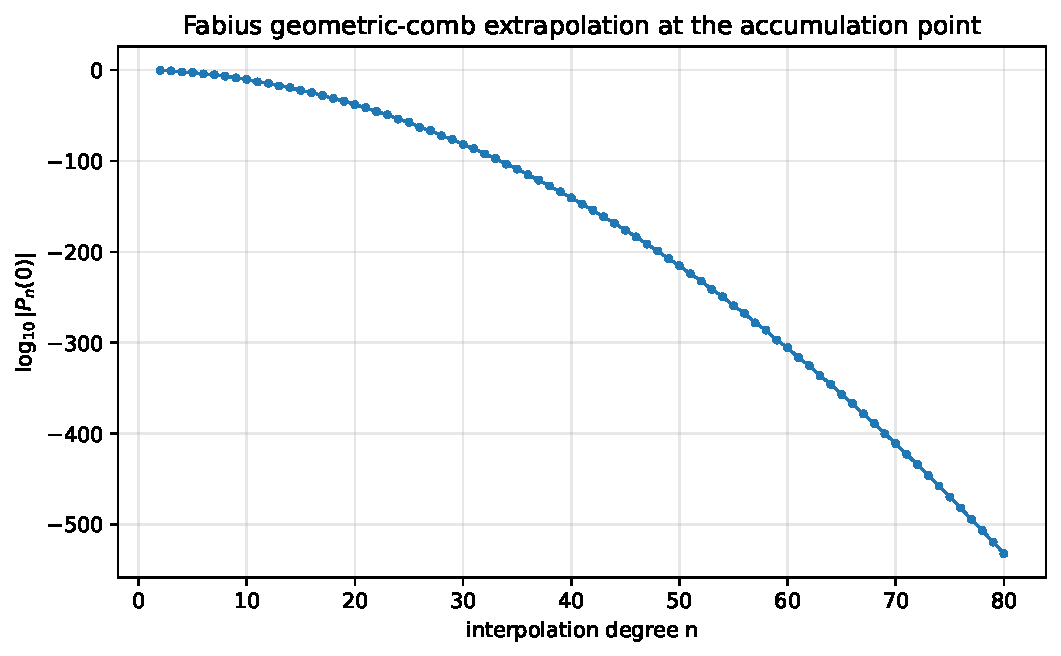
\includegraphics[width=0.87\textwidth]{fabius_endpoint_extrapolation.pdf}
\caption{Exact rational extrapolation errors at the accumulation point.  The
roughly parabolic graph on a logarithmic scale is consistent with the proved
$2^{-n^2/4+O(n)}$ bound.}
\label{fig:endpoint-extrapolation}
\end{figure}

\subsection{Divergence away from the comb}

At $x=1/3$, the first few interpolants look innocuous:
\[
 P_5(1/3)\approx0.1746,
 \qquad
 P_{10}(1/3)\approx0.2503.
\]
The later values are enormous:
\begin{center}
\begin{tabular}{r r}
\toprule
$n$ & $\log_{10}(1+|P_n(1/3)|)$\\
\midrule
15 & $4.1921$\\
20 & $12.3248$\\
30 & $39.4610$\\
40 & $80.7599$\\
60 & $206.0893$\\
80 & $392.7146$\\
\bottomrule
\end{tabular}
\end{center}
This does not merely suggest divergence; \Cref{cor:fabius-convergence-set}
proves it at every off-comb nonzero point.

\begin{figure}[H]
\centering
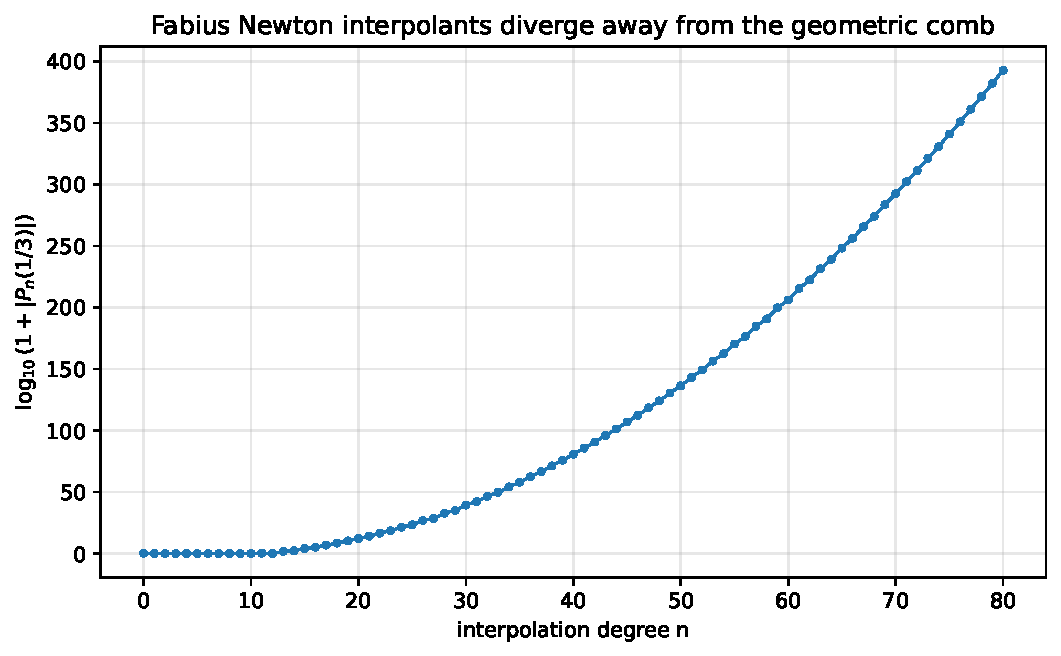
\includegraphics[width=0.87\textwidth]{fabius_newton_divergence.pdf}
\caption{Growth of the exact rational interpolants at $x=1/3$.  The small
values through degree $10$ are a long transient, not convergence.}
\label{fig:newton-divergence}
\end{figure}

\subsection{Quadratic growth of the Newton coefficients}

The normalized quantity $n^{-2}\log_2|A_n|$ rises slowly toward $1/4$ through
order $80$.  The slow approach is compatible with logarithmic and periodic
subquadratic corrections inherited from the endpoint asymptotics of the
Fabius function.

\begin{figure}[H]
\centering
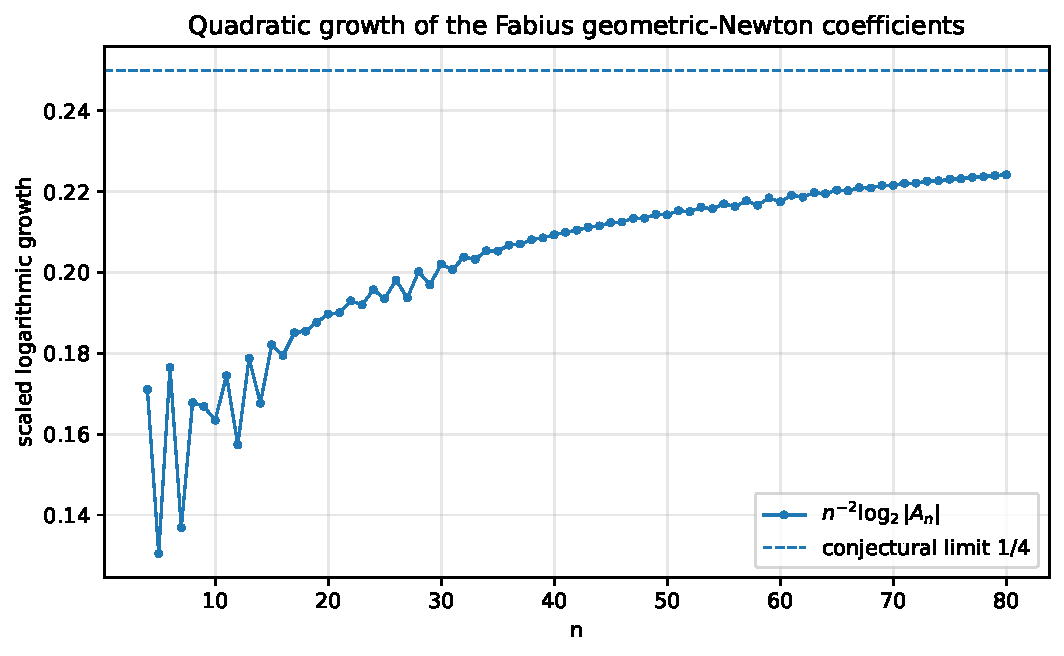
\includegraphics[width=0.87\textwidth]{fabius_newton_coefficient_growth.pdf}
\caption{Numerical evidence for \Cref{conj:quarter-exponent}.  The dashed line
is $1/4$; it is not fitted to the data.}
\label{fig:coefficient-growth}
\end{figure}

\subsection{Bounded row variation}

\Cref{thm:row-norm} predicts saturation at a finite $K(q)$ for every fixed
$q<1$.  The saturation is rapid for $q=1/4$ and $q=1/2$, while $q=3/4$
requires more levels and reaches a much larger condition number.

\begin{figure}[H]
\centering
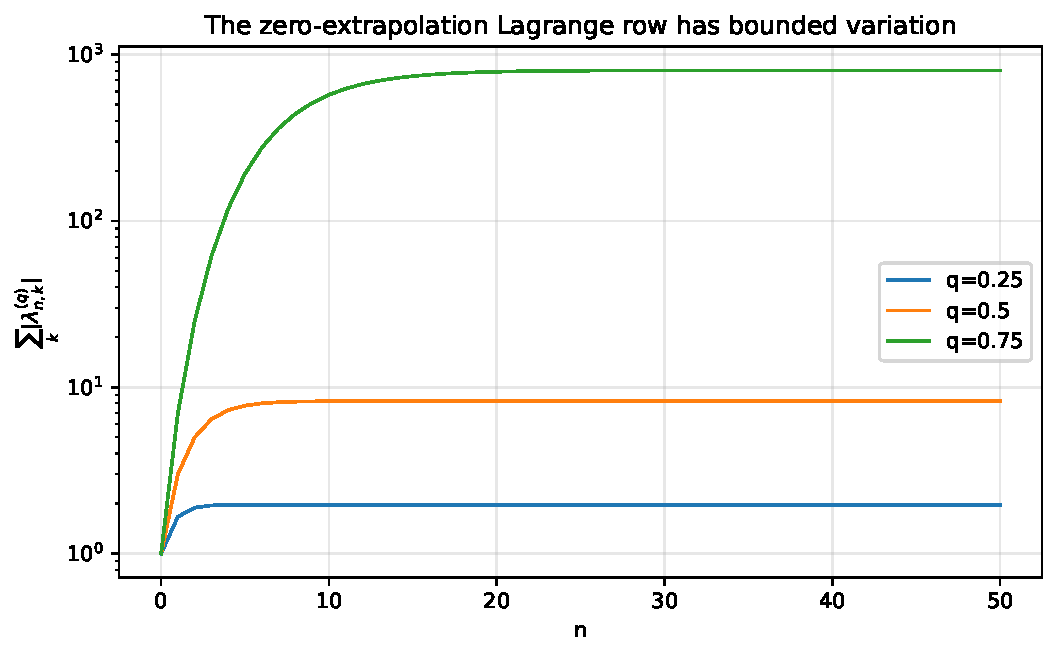
\includegraphics[width=0.87\textwidth]{lagrange_row_norm.pdf}
\caption{The exact row norm $(-q;q)_n/(q;q)_n$ on a logarithmic vertical
scale.  Fixed-ratio stability and the singular $q\to1$ limit are both visible.}
\label{fig:row-norm}
\end{figure}

\subsection{Reciprocal Rvachev product}

For $q=1/2$ and $\xi=0.37$,
\begin{align*}
 \widehat u(0.37)
 &\approx0.7319398291936895108374260130,\\
 \widehat u(0.37)^{-1}
 &\approx1.3662325236510323730502298892.
\end{align*}
The degree-$28$ reciprocal filter has absolute error about
$1.0\times10^{-100}$ at 100-digit working precision.

\begin{figure}[H]
\centering
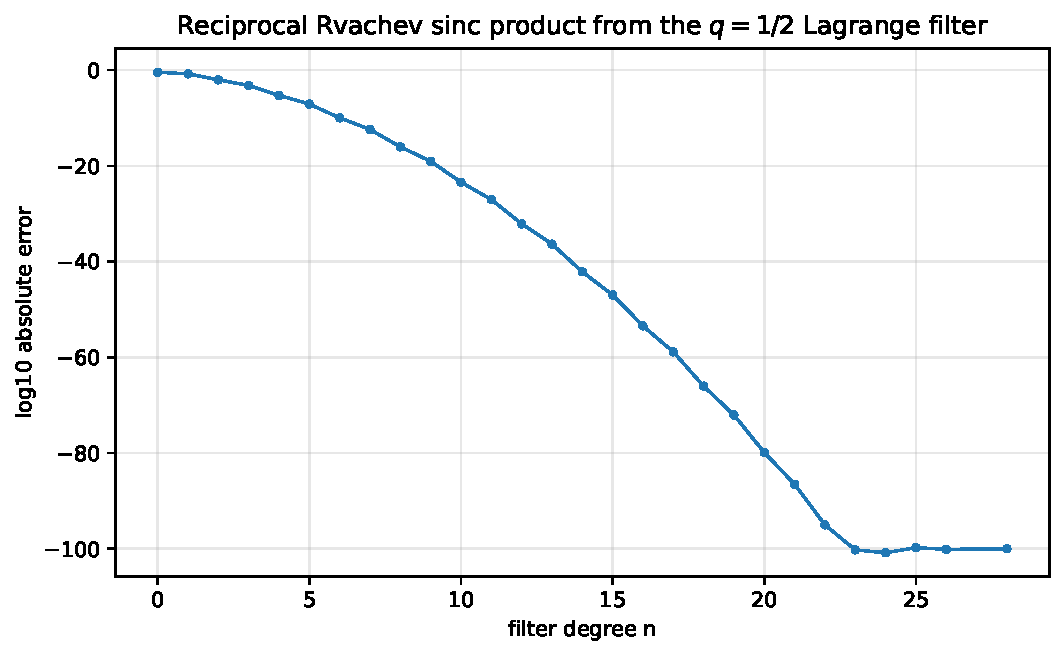
\includegraphics[width=0.87\textwidth]{rvachev_reciprocal_filter.pdf}
\caption{High-precision error in the reciprocal-product approximant
\eqref{eq:reciprocal-approximant}.  The combination of the Gaussian factor
$q^{\binom{n+1}{2}}$ and the factorial Taylor tail gives extremely rapid
convergence.}
\label{fig:rvachev-reciprocal}
\end{figure}

\section{Research frontiers}
\label{sec:frontiers}

The problems below are ordered from sharply formulated local questions to
broader structural programs.  None is needed for the proved results.

\subsection{Asymptotics of the Fabius Newton coefficients}

\Cref{conj:quarter-exponent} asks only for the leading quadratic exponent.  A
more informative target is a saddle-point expansion of
\eqref{eq:fabius-Gaussian-transform} or
\eqref{eq:newton-generating-factorization}.  The Gaussian coefficient favors
$j\approx n/2$, while $\mu_j/j!$ has its own lower-Lambert saddle and periodic
correction.  The interaction should produce a two-scale saddle problem.

\begin{problem}[Full coefficient asymptotic]
\label{prob:full-A-asymptotic}
Determine functions $c_2,c_1,c_{\log}$ and a bounded oscillatory term
$\Psi$ such that
\begin{equation}
 \log|A_n|
 =c_2n^2+c_1n\log n+c_{\log}n
 +\Psi(\vartheta_n)+o(1),
 \label{eq:full-A-asymptotic}
\end{equation}
with an explicit Lambert-type phase $\vartheta_n$.  Decide whether sign
changes and near-cancellations are controlled by the same periodic function
that occurs in the sharp Fabius endpoint asymptotic.
\end{problem}

A first rigorous step would be matching upper and lower bounds
$2^{n^2/4+o(n^2)}$.  The upper bound is already in
\Cref{cor:coefficient-upper}; a lower bound must prevent exponential-scale
cancellation in the alternating central block.

\subsection{Boundary-crossing formulas for \texorpdfstring{$q>1/2$}{q greater than 1/2}}

\begin{problem}[The supercritical comb-moment law]
\label{prob:qgt-half}
For $1/2<q<1$, derive a closed formula for $F_q(q^n)$ in terms of moments and
finite affine words generated by
\[
 x\mapsto x/q,
 \qquad
 x\mapsto(x-(1-q))/q.
\]
A satisfactory formula should specialize to \eqref{eq:comb-moment} when no
word crosses the reflected boundary, and should make the breakpoints in $q$
explicit.
\end{problem}

The number of admissible boundary words may change when polynomial relations
among $q$-powers are crossed.  This suggests a piecewise-algebraic structure
related to beta-expansions, but with continuous uniform digits rather than
Bernoulli digits.

\subsection{Confluent limits and roots of unity}

\begin{problem}[$q\to0$ confluent calculus]
\label{prob:q0-confluent}
Find a renormalized cardinal and Newton basis whose $q\to0$ limit separates the
infinitely many nodes collapsing at $0$.  Determine whether the correct limit
is a triangular mixture of value, derivative, and tail-quotient functionals.
\end{problem}

\begin{problem}[Cyclotomic geometric interpolation]
\label{prob:roots-unity}
When $q$ is a primitive $m$th root of unity, replace repeated nodes by a
canonical Hermite data set and factor the resulting confluent Vandermonde
matrix into cyclotomic analogues of $P_q$ and $D_{a,q}$.  The denominator-free
operator
$\prod_{j=1}^n(E_q-q^j)$ should survive as a periodic difference operator even
when normalized Lagrange weights do not.
\end{problem}

These limits may connect the present theory to divided powers, quantum groups
at roots of unity, and cyclic $q$-difference equations.

\subsection{Regularization near Fourier zeros}

\begin{problem}[Filtered finite parts at sinc zeros]
\label{prob:zero-regularization}
Let $\xi_0$ be a zero of $\widehat u_q$ of known multiplicity $m$.  Construct
from $R_{n,q}$ and its first $m$ derivatives a sequence converging to the
finite part of $1/\widehat u_q$ at $\xi_0$, with a bound uniform in a shrinking
neighborhood of the zero.
\end{problem}

Because every zero comes from explicit finite sinc factors, one can first
divide out the known local factor and then apply the geometric filter to the
nonvanishing tail.  The main issue is numerical cancellation when several
zero lattices overlap, as they do extensively at $q=1/2$.

\subsection{Exact Lebesgue functions below the finest node}

For $x=aq^\alpha$ with real $\alpha>n$, the cardinal signs are
$(-1)^{n-j}$, so the Lebesgue function is the explicit positive sum below.
The formula extends continuously to $\alpha=n$, where the target is the finest
node and the Lebesgue function equals $1$.
\begin{equation}
 \Lambda_n(aq^\alpha)=
 (q^{\alpha-n};q)_{n+1}
 \sum_{j=0}^n
 \frac{q^{\binom{n-j+1}{2}}}
 {(1-q^{\alpha-j})(q;q)_j(q;q)_{n-j}}.
 \label{eq:below-comb-lebesgue}
\end{equation}
At $\alpha=\infty$ it reduces to \eqref{eq:row-norm}.  It is natural to ask
whether the finite sum has a single basic-hypergeometric closed form and
whether $\Lambda_n$ is monotone on $[0,aq^n]$.

\begin{conjecture}[Maximum below the comb]
\label{conj:below-comb-lebesgue}
For $0<q<1$ and $a>0$,
\begin{equation}
 \max_{0\le x\le aq^n}\Lambda_n(x)=\Lambda_n(0)
 =\frac{(-q;q)_n}{(q;q)_n}.
 \label{eq:below-comb-max}
\end{equation}
\end{conjecture}

Low-degree symbolic and numerical checks support the claim, but a proof
appears to require a variation-diminishing or total-positivity argument rather
than termwise monotonicity.

\subsection{Flatness-adapted approximation spaces}

Polynomial interpolation fails off the comb for a structural reason.  The
basis must be changed, not merely evaluated more accurately.  Classical
geometric-knot spline constructions~\cite{KocakPhillips1994} provide one
nearby approximation-theoretic model, while Rvachev atoms add exact
$C^\infty$ compact support and endpoint flatness.

\begin{problem}[Rvachev-preconditioned comb interpolation]
\label{prob:rvachev-preconditioned}
Construct finite-dimensional spaces generated by scale-dependent Rvachev
atoms, for example
\[
 u(2^jx-r),\qquad 0\le j\le n,
\]
that interpolate the Fabius dyadic data and incorporate endpoint flatness.
Determine whether one can obtain convergence on $[0,1]$ while retaining exact
rational or algebraic coefficient formulas.
\end{problem}

The deconvolution formula \eqref{eq:q-Appell-cardinal} supplies an exact
preconditioner for each finite polynomial interpolant, but it cannot remove
the divergence because it reproduces the same polynomial.  A genuinely new
scheme must let the atom space grow in smoothness or scale, rather than merely
re-expressing $\mathbb P_n$.

\begin{problem}[Growing Hermite data]
\label{prob:growing-hermite}
At the tooth $2^{-j}$, include derivatives through an order $r_j$ that grows
with $j$.  Find the minimal growth of $r_j$ for which the Hermite interpolants
can converge to $F$ on a nontrivial interval.  Relate the threshold to the
sharp derivative and endpoint asymptotics of $F$.
\end{problem}

\subsection{Multivariate geometric meshes}

Schoenberg's one-dimensional problem has a triangular-mesh extension due to
Lee and Phillips~\cite{LeePhillips1988}.  The present operator and probability
viewpoints suggest several further versions.

\begin{problem}[Tensor and simplex filters]
\label{prob:multivariate}
For nodes
$(a_1q_1^{j_1},\ldots,a_dq_d^{j_d})$, develop tensor and total-degree
Lagrange filters with explicit multivariate Mellin symbols.  On a simplex-like
geometric mesh, identify the correct multivariate Gaussian coefficients and
complete homogeneous residuals.  Apply them to joint geometric-uniform laws
and tensor products of up-functions.
\end{problem}

The tensor case is immediate algebraically but may suffer severe anisotropic
conditioning.  The simplex case should involve $q$-multinomial coefficients
and may admit a probabilistic interpretation through flags of coordinate
subspaces.

\subsection{Adaptive ratios and asymptotic optimization}

The exact error factors make ratio selection an optimization problem.  Small
$q$ gives powerful Gaussian suppression but spreads the first nodes; $q$ near
$1$ resolves a local germ but causes the condition number
\eqref{eq:infinite-row-q1} to explode.

\begin{problem}[Optimal $q$ under noise]
\label{prob:optimal-q}
Suppose the data $f(aq^k)$ have absolute or relative noise of known scale and
$f$ belongs to a specified analytic, Gevrey, or endpoint-asymptotic class.
Minimize a rigorous sum of truncation and amplified-noise bounds over both
$q$ and $n$.  Determine whether the optimum has a universal scaling law as the
noise tends to zero.
\end{problem}

For the Fabius function, the superflat signal and the large off-comb
coefficients make this a nonstandard regularization problem; the optimum for
evaluating $F(0)$ need not resemble the optimum for reconstructing $F(x)$ at
$x>0$.

\subsection{Formal verification roadmap}

The finite algebra is particularly well suited to Lean because most identities
can be stated over a commutative ring before any division is introduced.  A
productive dependency order is:

\begin{enumerate}
\item prove the denominator-free nodal product and geometric Vandermonde
      factorization;
\item define the Gaussian Pascal matrix and prove
      \eqref{eq:q-pascal-inverse};
\item derive the barycentric denominator and general-target cardinal after
      adding field hypotheses;
\item define the dilation polynomial and prove the full polynomial identity
      \eqref{eq:lambda-characteristic};
\item obtain natural moment annihilation by evaluation, then extend to the
      analytic Mellin symbol in a complex-power layer;
\item formalize Jackson divided differences first for polynomials, then for
      functions with iterated $q$-derivatives;
\item prove the row-norm identity and Toeplitz regularity using summable
      reversed rows;
\item reuse the repository's geometric-uniform law to prove
      \eqref{eq:comb-moment};
\item instantiate at $q=1/2$ and connect to existing Fabius moments and
      Mersenne products;
\item formalize the superflat divergence theorem using a local power-series
      contradiction;
\item feed the existing sinc-product theorem through the analytic filter to
      obtain \Cref{thm:reciprocal-product}.
\end{enumerate}

The distinction between denominator-free polynomial statements and normalized
field statements should be maintained throughout.  It will make the later
root-of-unity and confluent developments substantially easier.

\section{Conclusions}
\label{sec:conclusion}

Interpolation on $a,aq,aq^2,\ldots$ is one of the places where ordinary
numerical analysis and $q$-analysis are literally the same theory written in
different coordinates.  The nodal polynomial is a $q$-Pochhammer symbol, the
Vandermonde factorization is Gaussian Pascal, the Newton coefficients are
Jackson derivatives, and the extrapolation row is a finite polynomial in the
dilation operator.  Its Mellin symbol
\[
 q^{ns}\frac{(q^{1-s};q)_n}{(q;q)_n}
\]
contains the entire exactness theory, including fractional and logarithmic
endpoint terms.

The accumulation point has a subtle status.  Fixed-ratio extrapolation to zero
is stable in the Toeplitz sense because the row norm tends to
$(-q;q)_\infty/(q;q)_\infty$.  Yet interpolation away from the comb is not a
reconstruction method for arbitrary smooth functions.  For nonzero superflat
data the Newton coefficients grow beyond every exponential scale, and the
interpolants diverge everywhere except on the sampled comb and at its limit.
The Fabius function realizes this theorem in an exact arithmetic setting.

The probabilistic family $X_q=(1-q)\sum q^jU_j$ completes the bridge.  Its
moments carry $1-q^n$ denominators, its CDF samples on the comb become
normalized moments for $q\le1/2$, and its centered density has the same
geometric sinc product that defines Rvachev's up-function at $q=1/2$.
Accordingly, the Gaussian filter acts on both sides: it converts Fabius samples
into Mersenne moment transforms, and it converts Rvachev tail products into a
reciprocal Fourier expansion.

The most promising next steps are a full saddle asymptotic for the Fabius
Newton coefficients, a boundary-word formula for $q>1/2$, and approximation
spaces that encode flatness from the outset.  Those problems sit precisely at
the interface of $q$-series, endpoint asymptotics, compactly supported smooth
atoms, and formally verified analysis.

\appendix

\section{Selected finite identities}
\label{app:finite-identities}

For quick reference, the principal finite formulas are collected here.

\begin{align*}
 \Omega_{n+1}(x)
 &=x^{n+1}(a/x;q)_{n+1},\\[0.3em]
 \Phi_k(x)
 &=(-a)^kq^{\binom k2}(x/a;q^{-1})_k,\\[0.3em]
 \Phi_k(aq^j)
 &=(-a)^kq^{\binom k2}(q;q)_k\qbinom jkq,\\[0.3em]
 \beta_{n,j}
 &=\frac{(-1)^jq^{-jn+\binom{j+1}{2}}}
 {a^n(q;q)_j(q;q)_{n-j}},\\[0.3em]
 \lambda_{n,j}^{(q)}
 &=\frac{(-1)^{n-j}q^{\binom{n-j+1}{2}}}
 {(q;q)_j(q;q)_{n-j}},\\[0.3em]
 \sum_{j=0}^n\lambda_{n,j}^{(q)}z^j
 &=\frac{\prod_{r=1}^n(z-q^r)}{(q;q)_n},\\[0.3em]
 f[a,aq,\ldots,aq^k]
 &=\frac{D_q^kf(a)}{[k]_q!},\\[0.3em]
 \sum_{j=0}^n|\lambda_{n,j}^{(q)}|
 &=\frac{(-q;q)_n}{(q;q)_n},\\[0.3em]
 M_{n,q}(s)
 &=q^{ns}\frac{(q^{1-s};q)_n}{(q;q)_n},\\[0.3em]
 F_q(q^n)
 &=\frac{q^{\binom{n+1}{2}}}{(1-q)^nn!}\E X_q^n
 \quad(0<q\le1/2),\\[0.3em]
 F(2^{-n})
 &=2^{-\binom n2}\frac{\mu_n}{n!},\\[0.3em]
 A_n
 &=\frac1{(1/2;1/2)_n}
 \sum_{j=0}^n(-1)^j\qbinom nj2\frac{\mu_j}{j!}.
\end{align*}

\section{Pseudocode for exact dyadic computation}
\label{app:pseudocode}

The following high-level algorithm uses rational arithmetic throughout.

\begin{lstlisting}[style=pythonstyle]
mu[0] = 1
M[0]  = 1
for n = 1..N:
    mu[n] = (sum_{k=0}^{n-1} binom(n,k)*mu[k]/(n-k+1)) / (2^n-1)
    M[n]  = M[n-1]*(2^n-1)

for n = 0..N:
    Fdyadic[n] = 2^(-n*(n-1)/2) * mu[n] / n!
    A[n] = 2^(n*(n+1)/2) *
           sum_{j=0}^n (-1)^j * mu[j] / (j!*M[j]*M[n-j])
    E[n] = sum_{j=0}^n (-1)^(n-j) * 2^j * mu[j]
           / (j!*M[j]*M[n-j])
\end{lstlisting}

The attached Python implementation additionally verifies all transforms by
independent formulas, evaluates Newton partial sums at rational targets, and
computes the high-precision Fourier-product experiment.

\section{Source map}
\label{app:source-map}

The repository files most directly related to this report are:

\begin{itemize}
\item \nolinkurl{Analysis/FabiusFunction/docs/semi-formalized-research-frontiers/drafts/exponents-and-q-series/q_pochhammer_q_binomial_monograph/q_pochhammer_q_binomial_monograph.tex},
which supplies the initial geometric Newton and exact-filter formulas;
\item \nolinkurl{Analysis/FabiusFunction/docs/Fabius_Function_and_Rvachev_Up/Fabius_Function_and_Rvachev_Up.tex}, the primary human-readable synthesis of
the formal Fabius development and geometric-uniform law;
\item \nolinkurl{Analysis/FabiusFunction/docs/semi-formalized-research-frontiers/drafts/representations/lagrange_rvachev_loop_report_v3/lagrange_rvachev_loop.tex}, which develops
finite Lagrange/Legendre/up-function synthesis and the deconvolution operator
used in \Cref{sec:up-synthesis-bridge}.
\end{itemize}

\begin{thebibliography}{99}

\bibitem{Arias2017Definition}
J.~Arias de Reyna,
\newblock \emph{An infinitely differentiable function with compact support:
definition and properties},
\newblock English translation of \emph{Rev. Real Acad. Cienc. Exact. Fis.
Natur. Madrid} \textbf{76} (1982), 21--38,
\newblock arXiv:1702.05442, 2017.

\bibitem{Arias2017Arithmetic}
J.~Arias de Reyna,
\newblock \emph{Arithmetic of the Fabius function},
\newblock arXiv:1702.06487, 2017.

\bibitem{DLMF17}
NIST Digital Library of Mathematical Functions,
\newblock Chapter 17, \emph{$q$-Hypergeometric and Related Functions},
\newblock especially Section 17.2, release 1.2.7 of 15 June 2026.

\bibitem{Fabius1966}
J.~Fabius,
\newblock A probabilistic example of a nowhere analytic $C^\infty$-function,
\newblock \emph{Zeitschrift f\"ur Wahrscheinlichkeitstheorie und Verwandte
Gebiete} \textbf{5} (1966), 173--174,
\newblock doi:10.1007/BF00536652.

\bibitem{GasperRahman2004}
G.~Gasper and M.~Rahman,
\newblock \emph{Basic Hypergeometric Series}, second edition,
\newblock Encyclopedia of Mathematics and its Applications 96,
Cambridge University Press, 2004.

\bibitem{Haugland2016}
J.~K.~Haugland,
\newblock \emph{Evaluating the Fabius function},
\newblock arXiv:1609.07999, 2016, revised 2020.

\bibitem{JessenWintner1935}
B.~Jessen and A.~Wintner,
\newblock Distribution functions and the Riemann zeta function,
\newblock \emph{Transactions of the American Mathematical Society}
\textbf{38} (1935), 48--88.

\bibitem{KacCheung2002}
V.~Kac and P.~Cheung,
\newblock \emph{Quantum Calculus},
\newblock Universitext, Springer, 2002.

\bibitem{KocakPhillips1994}
Z.~F.~Ko\c{c}ak and G.~M.~Phillips,
\newblock B-splines with geometric knot spacings,
\newblock \emph{BIT Numerical Mathematics} \textbf{34} (1994), 388--399,
\newblock doi:10.1007/BF01935648.


\bibitem{LeePhillips1988}
S.~L.~Lee and G.~M.~Phillips,
\newblock Polynomial interpolation at points of a geometric mesh on a triangle,
\newblock \emph{Proceedings of the Royal Society of Edinburgh Section A:
Mathematics} \textbf{108} (1988), 75--87,
\newblock doi:10.1017/S0308210500026536.

\bibitem{ProveItFabius}
V.~Reshetnikov,
\newblock \emph{The Fabius Function and Rvachev's Up-Function: Exact
arithmetic, probability, Fourier analysis, and corrected sharp asymptotics},
\newblock \texttt{ProveIt} repository,
\nolinkurl{Analysis/FabiusFunction/docs/Fabius_Function_and_Rvachev_Up},
repository snapshot inspected 30 August 2026.

\bibitem{ProveItLagrangeLoop}
V.~Reshetnikov,
\newblock \emph{Lagrange--Legendre--Rvachev loop report},
\newblock \texttt{ProveIt} repository,
\nolinkurl{Analysis/FabiusFunction/docs/semi-formalized-research-frontiers/drafts/representations/lagrange_rvachev_loop_report_v3},
repository snapshot inspected 30 August 2026.

\bibitem{Schoenberg1981}
I.~J.~Schoenberg,
\newblock On polynomial interpolation at the points of a geometric
progression,
\newblock \emph{Proceedings of the Royal Society of Edinburgh Section A:
Mathematics} \textbf{90} (1981), 195--207,
\newblock doi:10.1017/S0308210500015456.

\end{thebibliography}

\end{document}
